%%%%%%%%%%%%%%%%%%%%%%%%%%%%%%%%%%%%%%%%%%%%%%%%%%%%%%%%%%%%%%%%%%%%%%%%%%%%%%%%
\subsection{Πειραματική διαδικασία}
\label{subsection:02_03_04:01}

Προκειμένου να ελεγχθεί η υπόθεση \ref{hypothesis:02_03:01} και η
αποτελεσματικότητα της προτεινόμενης μεθόδου πραγματοποιούμε προσομοιώσεις και
πειράματα σε διαφορετικά---δομημένα και αδόμητα---περιβάλλοντα, και υπό
διαφορετικές αναλύσεις των χαρτών τους.  Προκειμένου να ελεγχθεί η ευρωστία της
προτεινόμενης μεθόδου στην επίδραση διαταραχών, εκτελούμε την πειραματική
διαδικασία έναντι επιπέδων θορύβων που φέρουν διαθέσιμοι εμπορικά αισθητήρες.
Το ρομπότ που χρησιμοποιήθηκε σε όλες τις προσομοιώσεις ήταν ένα Turtlebot
v.$2$, εξοπλισμένο με έναν αισθητήρα lidar μέγιστου ακτινικού εύρους $10.0$
μέτρων, ο οποίος αναφέρει $N_s=720$ μετρήσεις δύο διαστάσεων, σε γωνιακό εύρος
$360$ μοιρών. Η μέγιστη ανιχνευόμενη ακτινική απόσταση ορίστηκε σε αυτή την
τιμή προκειμένου να περιορίζεται ο όγκος των πληροφοριών που είναι διαθέσιμες
σε κάθε μέθοδο ευθυγράμμισης, ώστε να ελεγχθεί ταυτόχρονα η ευρωστία τους στην
απουσία πληροφοριών, πέραν αυτής που αφορά στην αβεβαιότητα τους. Για να
ελεγχθεί η επίδοση της προτεινόμενης μεθόδου σε πραγματικές συνθήκες
χρησιμοποιήθηκε ο αισθητήρας YDLIDAR TG30. Η μέγιστη ανιχνευόμενη ακτινική
απόστασή του είναι $30.0$ m, και ο αριθμός των εκπεμπόμενων ακτίνων είναι $N_s
= 2019$ \cite{ydlidar}. Παράλληλα, η επίδοση της προτεινόμενης μεθόδου PGL-FMIC
αντιπαραβάλλεται με τον αλγόριθμο PLICP σε μια προσπάθεια να καταγραφούν τα
συγκριτικά πλεονεκτήματα και μειονεκτήματα των δύο μεθόδων. Ο τρόπος με τον
οποίο ο PLICP μπορεί να χρησιμοποιηθεί για την επίλυση του προβλήματος της
εκτίμησης της στάσης ενός ρομπότ του πεδίου εφαρμογής \ref{scope} βάσει
καθολικής αβεβαιότητος περιγράφηκε στην ενότητα \ref{subsection:02_02_05:02}.

Και οι δύο αλγόριθμοι δοκιμάστηκαν σε πέντε προσομοιωμένα περιβάλλοντα, τα
οποία ονομάζονται CORRIDOR, HOME, WAREHOUSE, WILLOWGARAGE, και LANDFILL, για
συνολικά $38$ στάσεις ρομπότ, και για τρία επίπεδα θορύβου του αισθητήρα
απόστασης για κάθε στάση. Ο θόρυβος που διαταράσσει τις μετρήσεις του είναι
κανονικά κατανεμημένος με τυπική απόκλιση $d \in \mathcal{D} = \{0.01, 0.02,
0.05\}$ m και μηδενική μέση τιμή. Οι αποστάσεις των εικονικών σαρώσεων
διαταράσσονται αναλογικά με την παραποίηση του περιβάλλοντος στο οποίο
αντιστοιχεί ο χάρτης.  Οι χάρτες των περιβαλλόντων CORRIDOR ($\bm{M}_C$), HOME
($\bm{M}_H$), WAREHOUSE ($\bm{M}_W$), και LANDFILL ($\bm{M}_L$) κατασκευάστηκαν
με το ίδιο ρομπότ, του οποίου οι μετρήσεις διαταράσσονται από θόρυβο κανονικά
κατανεμημένο, με μηδενική μέση τιμή, και τυπική απόκλιση $d = 0.01$ m. Το
περιβάλλον από το οποίο δημιουργήθηκε ο χάρτης $\bm{M}_L$ κατασκευάστηκε από
μοντέλα του συνόλου δεδομένων \texttt{3DGEMS} \cite{Rasouli2017}, ενώ ο χάρτης
$\bm{M}_G$ λήφθηκε από το \cite{willow_map}.  Οι δύο αλγόριθμοι δοκιμάστηκαν
επίσης σε ένα πραγματικό περιβάλλον, σε $11$ πραγματικές στάσεις του ρομπότ. Τα
πειράματα σε πραγματικές συνθήκες πραγματοποιήθηκαν στο Εργαστήριο
Αρχιτεκτονικής Συστημάτων Υπολογιστών (CSAL) του Αριστοτελείου Πανεπιστημίου
Θεσσαλονίκης (ΑΠΘ). Ο χάρτης του CSAL $\bm{M}_A$ κατασκευάστηκε με τη χρήση
ενός Turtlebot v.$2$, το οποίο απεικονίζεται μαζί με τον πανοραμικό αισθητήρα
lidar που φέρει στην εικόνα \ref{img:02_03_04:tb_yd}.

\begin{figure}\centering
  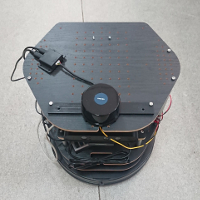
\includegraphics[scale=1]{./figures/parts/02/chapters/03/sections/04/tb_yd.jpg}
  \caption{\small Το ρομπότ τύπου turtlebot και ο πανοραμικός αισθητήρας
           αποστάσεων τύπου LIDAR δισδιάστατων μετρήσεων που χρησιμοποιήθηκαν
           κατά την πειραματική διαδικασία}
  \label{img:02_03_04:tb_yd}
\label{}
\end{figure}

Για τον προσδιορισμό κάθε στάσης του ρομπότ κάθε προσομοίωση πραγματοποιήθηκε
$N = 100$ φορές για κάθε αλγόριθμο για λόγους αξιοπιστίας των συμπερασμάτων. Ο
συνολικός αριθμός των προσομοιώσεων που πραγματοποιήθηκαν για κάθε μέθοδο ήταν
επομένως $ 38 \times 100 \times 3 \sim \mathcal{O}(4)$.  Για τον προσδιορισμό
κάθε στάσης του ρομπότ στο πραγματικό περιβάλλον κάθε πείραμα πραγματοποιήθηκε
$N = 5$ φορές.

Τα πέντε προσομοιωμένα και το ένα πραγματικό περιβάλλον απεικονίζονται στo
σχήμα \ref{fig:02_03_04:maps_sim}. To σχήμα \ref{fig:02_03_04:maps_sim}(α')
απεικονίζει ένα απλό και σχεδόν συμμετρικό περιβάλλον που χρησιμοποιείται για
προκαταρκτική αξιολόγηση και σκοπούς διάκρισης στάσεων λόγω της συμμετρίας του.
Το σχήμα \ref{fig:02_03_04:maps_sim}(β') απεικονίζει ένα τυπικό οικιακό ή
εμπορικό χώρο διάσπαρτο από καρέκλες, τραπέζια, στήλες, και ορθογώνια έπιπλα.
Το σχήμα \ref{fig:02_03_04:maps_sim}(γ') απεικονίζει ένα τυπικό περιβάλλον
αποθήκης, με μεγάλους ανοιχτούς χώρους, στους οποίους δοκιμάζεται η ικανότητα
των μεθόδων να ανταπεξέλθουν σε ελλιπείς πληροφορίες. Στο σχήμα
\ref{fig:02_03_04:maps_sim}(δ') απεικονίζεται ένα μεγάλο συγκρότημα που
ομοιάζει με σύμπλεγμα γραφείων, όπου οι μέθοδοι αξιολογούνται περισσότερο
προσεκτικά ως προς την ικανότητά τους να επιλύουν ασάφειες στάσης λόγω
επανάληψης της γεωμετρίας των μερών του. Το σχήμα
\ref{fig:02_03_04:maps_sim}(στ') απεικονίζει ένα μη δομημένο περιβάλλον
παρόμοιο με αυτό μίας χωματερής, το οποίο χρησιμοποιείται για να διαπιστωθεί η
εγκυρότητα του ισχυρισμού ότι η επίδοση του PGL-FMIC δεν κάνει διάκριση μεταξύ
δομημένων και μη περιβαλλόντων. Οι χάρτες των δύο τελευταίων περιβαλλόντων
(WILLOWGARAGE και LANDFILL) έχουν ανάλυση $0.05\times0.05$ m$^2$, ενώ εκείνοι
των άλλων τριών $0.01\times0.01$ m$^2$. Ο χάρτης του εργαστηρίου CSAL
απεικονίζεται στο σχήμα \ref{fig:02_03_04:maps_sim}(ε') και η ανάλυση του είναι
$0.05\times0.05$ m$^2$.

\begin{figure}
  \begin{subfigure}{0.5\linewidth}
    % GNUPLOT: LaTeX picture with Postscript
\begingroup
  \makeatletter
  \providecommand\color[2][]{%
    \GenericError{(gnuplot) \space\space\space\@spaces}{%
      Package color not loaded in conjunction with
      terminal option `colourtext'%
    }{See the gnuplot documentation for explanation.%
    }{Either use 'blacktext' in gnuplot or load the package
      color.sty in LaTeX.}%
    \renewcommand\color[2][]{}%
  }%
  \providecommand\includegraphics[2][]{%
    \GenericError{(gnuplot) \space\space\space\@spaces}{%
      Package graphicx or graphics not loaded%
    }{See the gnuplot documentation for explanation.%
    }{The gnuplot epslatex terminal needs graphicx.sty or graphics.sty.}%
    \renewcommand\includegraphics[2][]{}%
  }%
  \providecommand\rotatebox[2]{#2}%
  \@ifundefined{ifGPcolor}{%
    \newif\ifGPcolor
    \GPcolorfalse
  }{}%
  \@ifundefined{ifGPblacktext}{%
    \newif\ifGPblacktext
    \GPblacktexttrue
  }{}%
  % define a \g@addto@macro without @ in the name:
  \let\gplgaddtomacro\g@addto@macro
  % define empty templates for all commands taking text:
  \gdef\gplfronttext{}%
  \gdef\gplfronttext{}%
  \makeatother
  \ifGPblacktext
    % no textcolor at all
    \def\colorrgb#1{}%
    \def\colorgray#1{}%
  \else
    % gray or color?
    \ifGPcolor
      \def\colorrgb#1{\color[rgb]{#1}}%
      \def\colorgray#1{\color[gray]{#1}}%
      \expandafter\def\csname LTw\endcsname{\color{white}}%
      \expandafter\def\csname LTb\endcsname{\color{black}}%
      \expandafter\def\csname LTa\endcsname{\color{black}}%
      \expandafter\def\csname LT0\endcsname{\color[rgb]{1,0,0}}%
      \expandafter\def\csname LT1\endcsname{\color[rgb]{0,1,0}}%
      \expandafter\def\csname LT2\endcsname{\color[rgb]{0,0,1}}%
      \expandafter\def\csname LT3\endcsname{\color[rgb]{1,0,1}}%
      \expandafter\def\csname LT4\endcsname{\color[rgb]{0,1,1}}%
      \expandafter\def\csname LT5\endcsname{\color[rgb]{1,1,0}}%
      \expandafter\def\csname LT6\endcsname{\color[rgb]{0,0,0}}%
      \expandafter\def\csname LT7\endcsname{\color[rgb]{1,0.3,0}}%
      \expandafter\def\csname LT8\endcsname{\color[rgb]{0.5,0.5,0.5}}%
    \else
      % gray
      \def\colorrgb#1{\color{black}}%
      \def\colorgray#1{\color[gray]{#1}}%
      \expandafter\def\csname LTw\endcsname{\color{white}}%
      \expandafter\def\csname LTb\endcsname{\color{black}}%
      \expandafter\def\csname LTa\endcsname{\color{black}}%
      \expandafter\def\csname LT0\endcsname{\color{black}}%
      \expandafter\def\csname LT1\endcsname{\color{black}}%
      \expandafter\def\csname LT2\endcsname{\color{black}}%
      \expandafter\def\csname LT3\endcsname{\color{black}}%
      \expandafter\def\csname LT4\endcsname{\color{black}}%
      \expandafter\def\csname LT5\endcsname{\color{black}}%
      \expandafter\def\csname LT6\endcsname{\color{black}}%
      \expandafter\def\csname LT7\endcsname{\color{black}}%
      \expandafter\def\csname LT8\endcsname{\color{black}}%
    \fi
  \fi
  \setlength{\unitlength}{0.0500bp}%
  \begin{picture}(4000.00,4000.00)%
    \gplgaddtomacro\gplfronttext{%
      \colorrgb{0.00,0.00,0.00}%
      \put(388,877){\makebox(0,0)[r]{\strut{}4}}%
      \colorrgb{0.00,0.00,0.00}%
      \put(388,1354){\makebox(0,0)[r]{\strut{}6}}%
      \colorrgb{0.00,0.00,0.00}%
      \put(388,1831){\makebox(0,0)[r]{\strut{}8}}%
      \colorrgb{0.00,0.00,0.00}%
      \put(388,2307){\makebox(0,0)[r]{\strut{}10}}%
      \colorrgb{0.00,0.00,0.00}%
      \put(388,2784){\makebox(0,0)[r]{\strut{}12}}%
      \colorrgb{0.00,0.00,0.00}%
      \put(388,3261){\makebox(0,0)[r]{\strut{}14}}%
      \colorrgb{0.00,0.00,0.00}%
      \put(520,419){\makebox(0,0){\strut{}2}}%
      \colorrgb{0.00,0.00,0.00}%
      \put(997,419){\makebox(0,0){\strut{}4}}%
      \colorrgb{0.00,0.00,0.00}%
      \put(1474,419){\makebox(0,0){\strut{}6}}%
      \colorrgb{0.00,0.00,0.00}%
      \put(1950,419){\makebox(0,0){\strut{}8}}%
      \colorrgb{0.00,0.00,0.00}%
      \put(2427,419){\makebox(0,0){\strut{}10}}%
      \colorrgb{0.00,0.00,0.00}%
      \put(2904,419){\makebox(0,0){\strut{}12}}%
      \colorrgb{0.00,0.00,0.00}%
      \put(3381,419){\makebox(0,0){\strut{}14}}%
      \colorrgb{0.00,0.00,0.00}%
      \put(-118,2069){\rotatebox{90}{\makebox(0,0){\strut{}$y$ [m]}}}%
      \colorrgb{0.00,0.00,0.00}%
      \put(2069,89){\makebox(0,0){\strut{}$x$ [m]}}%
    }%
    \gplgaddtomacro\gplfronttext{%
    }%
    \put(0,0){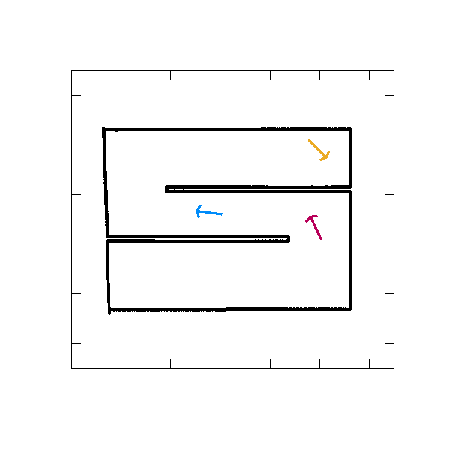
\includegraphics{./figures/parts/02/chapters/03/sections/04/map_corridor}}%
    \gplfronttext
  \end{picture}%
\endgroup

    %\caption{\small Ο χάρτης $\bm{M}_C$ του περιβάλλοντος CORRIDOR}
    \label{fig:02_03_04:map_corridor}
  \end{subfigure}%
  \begin{subfigure}{0.5\linewidth}
    % GNUPLOT: LaTeX picture with Postscript
\begingroup
  \makeatletter
  \providecommand\color[2][]{%
    \GenericError{(gnuplot) \space\space\space\@spaces}{%
      Package color not loaded in conjunction with
      terminal option `colourtext'%
    }{See the gnuplot documentation for explanation.%
    }{Either use 'blacktext' in gnuplot or load the package
      color.sty in LaTeX.}%
    \renewcommand\color[2][]{}%
  }%
  \providecommand\includegraphics[2][]{%
    \GenericError{(gnuplot) \space\space\space\@spaces}{%
      Package graphicx or graphics not loaded%
    }{See the gnuplot documentation for explanation.%
    }{The gnuplot epslatex terminal needs graphicx.sty or graphics.sty.}%
    \renewcommand\includegraphics[2][]{}%
  }%
  \providecommand\rotatebox[2]{#2}%
  \@ifundefined{ifGPcolor}{%
    \newif\ifGPcolor
    \GPcolorfalse
  }{}%
  \@ifundefined{ifGPblacktext}{%
    \newif\ifGPblacktext
    \GPblacktexttrue
  }{}%
  % define a \g@addto@macro without @ in the name:
  \let\gplgaddtomacro\g@addto@macro
  % define empty templates for all commands taking text:
  \gdef\gplfronttext{}%
  \gdef\gplfronttext{}%
  \makeatother
  \ifGPblacktext
    % no textcolor at all
    \def\colorrgb#1{}%
    \def\colorgray#1{}%
  \else
    % gray or color?
    \ifGPcolor
      \def\colorrgb#1{\color[rgb]{#1}}%
      \def\colorgray#1{\color[gray]{#1}}%
      \expandafter\def\csname LTw\endcsname{\color{white}}%
      \expandafter\def\csname LTb\endcsname{\color{black}}%
      \expandafter\def\csname LTa\endcsname{\color{black}}%
      \expandafter\def\csname LT0\endcsname{\color[rgb]{1,0,0}}%
      \expandafter\def\csname LT1\endcsname{\color[rgb]{0,1,0}}%
      \expandafter\def\csname LT2\endcsname{\color[rgb]{0,0,1}}%
      \expandafter\def\csname LT3\endcsname{\color[rgb]{1,0,1}}%
      \expandafter\def\csname LT4\endcsname{\color[rgb]{0,1,1}}%
      \expandafter\def\csname LT5\endcsname{\color[rgb]{1,1,0}}%
      \expandafter\def\csname LT6\endcsname{\color[rgb]{0,0,0}}%
      \expandafter\def\csname LT7\endcsname{\color[rgb]{1,0.3,0}}%
      \expandafter\def\csname LT8\endcsname{\color[rgb]{0.5,0.5,0.5}}%
    \else
      % gray
      \def\colorrgb#1{\color{black}}%
      \def\colorgray#1{\color[gray]{#1}}%
      \expandafter\def\csname LTw\endcsname{\color{white}}%
      \expandafter\def\csname LTb\endcsname{\color{black}}%
      \expandafter\def\csname LTa\endcsname{\color{black}}%
      \expandafter\def\csname LT0\endcsname{\color{black}}%
      \expandafter\def\csname LT1\endcsname{\color{black}}%
      \expandafter\def\csname LT2\endcsname{\color{black}}%
      \expandafter\def\csname LT3\endcsname{\color{black}}%
      \expandafter\def\csname LT4\endcsname{\color{black}}%
      \expandafter\def\csname LT5\endcsname{\color{black}}%
      \expandafter\def\csname LT6\endcsname{\color{black}}%
      \expandafter\def\csname LT7\endcsname{\color{black}}%
      \expandafter\def\csname LT8\endcsname{\color{black}}%
    \fi
  \fi
  \setlength{\unitlength}{0.0500bp}%
  \begin{picture}(4000.00,4000.00)%
    \gplgaddtomacro\gplfronttext{%
      \colorrgb{0.00,0.00,0.00}%
      \put(388,900){\makebox(0,0)[r]{\strut{}5}}%
      \colorrgb{0.00,0.00,0.00}%
      \put(388,1408){\makebox(0,0)[r]{\strut{}10}}%
      \colorrgb{0.00,0.00,0.00}%
      \put(388,1917){\makebox(0,0)[r]{\strut{}15}}%
      \colorrgb{0.00,0.00,0.00}%
      \put(388,2425){\makebox(0,0)[r]{\strut{}20}}%
      \colorrgb{0.00,0.00,0.00}%
      \put(388,2933){\makebox(0,0)[r]{\strut{}25}}%
      \colorrgb{0.00,0.00,0.00}%
      \put(388,3441){\makebox(0,0)[r]{\strut{}30}}%
      \colorrgb{0.00,0.00,0.00}%
      \put(571,477){\makebox(0,0){\strut{}10}}%
      \colorrgb{0.00,0.00,0.00}%
      \put(1079,477){\makebox(0,0){\strut{}15}}%
      \colorrgb{0.00,0.00,0.00}%
      \put(1587,477){\makebox(0,0){\strut{}20}}%
      \colorrgb{0.00,0.00,0.00}%
      \put(2095,477){\makebox(0,0){\strut{}25}}%
      \colorrgb{0.00,0.00,0.00}%
      \put(2603,477){\makebox(0,0){\strut{}30}}%
      \colorrgb{0.00,0.00,0.00}%
      \put(3111,477){\makebox(0,0){\strut{}35}}%
      \colorrgb{0.00,0.00,0.00}%
      \put(3619,477){\makebox(0,0){\strut{}40}}%
      \colorrgb{0.00,0.00,0.00}%
      \put(-118,2069){\rotatebox{90}{\makebox(0,0){\strut{}$y$ [m]}}}%
      \colorrgb{0.00,0.00,0.00}%
      \put(2069,147){\makebox(0,0){\strut{}$x$ [m]}}%
      \put(2000,3700){\makebox(0,0){HOME}}%
    }%
    \gplgaddtomacro\gplfronttext{%
    }%
    \put(0,0){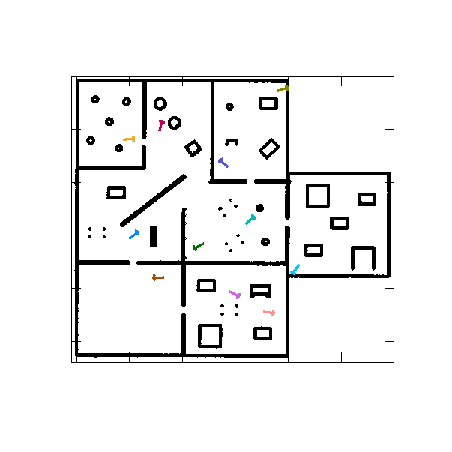
\includegraphics{./figures/parts/02/chapters/03/sections/04/map_home}}%
    \gplfronttext
  \end{picture}%
\endgroup

    %\caption{\small Ο χάρτης $\bm{M}_H$ του περιβάλλοντος HOME}
    \label{fig:02_03_04:map_home}
  \end{subfigure}\\
  \begin{subfigure}{0.5\linewidth}
    \vspace{0.5cm}
    % GNUPLOT: LaTeX picture with Postscript
\begingroup
  \makeatletter
  \providecommand\color[2][]{%
    \GenericError{(gnuplot) \space\space\space\@spaces}{%
      Package color not loaded in conjunction with
      terminal option `colourtext'%
    }{See the gnuplot documentation for explanation.%
    }{Either use 'blacktext' in gnuplot or load the package
      color.sty in LaTeX.}%
    \renewcommand\color[2][]{}%
  }%
  \providecommand\includegraphics[2][]{%
    \GenericError{(gnuplot) \space\space\space\@spaces}{%
      Package graphicx or graphics not loaded%
    }{See the gnuplot documentation for explanation.%
    }{The gnuplot epslatex terminal needs graphicx.sty or graphics.sty.}%
    \renewcommand\includegraphics[2][]{}%
  }%
  \providecommand\rotatebox[2]{#2}%
  \@ifundefined{ifGPcolor}{%
    \newif\ifGPcolor
    \GPcolorfalse
  }{}%
  \@ifundefined{ifGPblacktext}{%
    \newif\ifGPblacktext
    \GPblacktexttrue
  }{}%
  % define a \g@addto@macro without @ in the name:
  \let\gplgaddtomacro\g@addto@macro
  % define empty templates for all commands taking text:
  \gdef\gplfronttext{}%
  \gdef\gplfronttext{}%
  \makeatother
  \ifGPblacktext
    % no textcolor at all
    \def\colorrgb#1{}%
    \def\colorgray#1{}%
  \else
    % gray or color?
    \ifGPcolor
      \def\colorrgb#1{\color[rgb]{#1}}%
      \def\colorgray#1{\color[gray]{#1}}%
      \expandafter\def\csname LTw\endcsname{\color{white}}%
      \expandafter\def\csname LTb\endcsname{\color{black}}%
      \expandafter\def\csname LTa\endcsname{\color{black}}%
      \expandafter\def\csname LT0\endcsname{\color[rgb]{1,0,0}}%
      \expandafter\def\csname LT1\endcsname{\color[rgb]{0,1,0}}%
      \expandafter\def\csname LT2\endcsname{\color[rgb]{0,0,1}}%
      \expandafter\def\csname LT3\endcsname{\color[rgb]{1,0,1}}%
      \expandafter\def\csname LT4\endcsname{\color[rgb]{0,1,1}}%
      \expandafter\def\csname LT5\endcsname{\color[rgb]{1,1,0}}%
      \expandafter\def\csname LT6\endcsname{\color[rgb]{0,0,0}}%
      \expandafter\def\csname LT7\endcsname{\color[rgb]{1,0.3,0}}%
      \expandafter\def\csname LT8\endcsname{\color[rgb]{0.5,0.5,0.5}}%
    \else
      % gray
      \def\colorrgb#1{\color{black}}%
      \def\colorgray#1{\color[gray]{#1}}%
      \expandafter\def\csname LTw\endcsname{\color{white}}%
      \expandafter\def\csname LTb\endcsname{\color{black}}%
      \expandafter\def\csname LTa\endcsname{\color{black}}%
      \expandafter\def\csname LT0\endcsname{\color{black}}%
      \expandafter\def\csname LT1\endcsname{\color{black}}%
      \expandafter\def\csname LT2\endcsname{\color{black}}%
      \expandafter\def\csname LT3\endcsname{\color{black}}%
      \expandafter\def\csname LT4\endcsname{\color{black}}%
      \expandafter\def\csname LT5\endcsname{\color{black}}%
      \expandafter\def\csname LT6\endcsname{\color{black}}%
      \expandafter\def\csname LT7\endcsname{\color{black}}%
      \expandafter\def\csname LT8\endcsname{\color{black}}%
    \fi
  \fi
  \setlength{\unitlength}{0.0500bp}%
  \begin{picture}(4000.00,5000.00)%
    \gplgaddtomacro\gplfronttext{%
      \colorrgb{0.00,0.00,0.00}%
      \put(870,550){\makebox(0,0)[r]{\strut{}0}}%
      \colorrgb{0.00,0.00,0.00}%
      \put(870,1035){\makebox(0,0)[r]{\strut{}5}}%
      \colorrgb{0.00,0.00,0.00}%
      \put(870,1520){\makebox(0,0)[r]{\strut{}10}}%
      \colorrgb{0.00,0.00,0.00}%
      \put(870,2005){\makebox(0,0)[r]{\strut{}15}}%
      \colorrgb{0.00,0.00,0.00}%
      \put(870,2490){\makebox(0,0)[r]{\strut{}20}}%
      \colorrgb{0.00,0.00,0.00}%
      \put(870,2975){\makebox(0,0)[r]{\strut{}25}}%
      \colorrgb{0.00,0.00,0.00}%
      \put(870,3460){\makebox(0,0)[r]{\strut{}30}}%
      \colorrgb{0.00,0.00,0.00}%
      \put(870,3945){\makebox(0,0)[r]{\strut{}35}}%
      \colorrgb{0.00,0.00,0.00}%
      \put(870,4430){\makebox(0,0)[r]{\strut{}40}}%
      \colorrgb{0.00,0.00,0.00}%
      \put(1002,330){\makebox(0,0){\strut{}0}}%
      \colorrgb{0.00,0.00,0.00}%
      \put(1487,330){\makebox(0,0){\strut{}5}}%
      \colorrgb{0.00,0.00,0.00}%
      \put(1972,330){\makebox(0,0){\strut{}10}}%
      \colorrgb{0.00,0.00,0.00}%
      \put(2457,330){\makebox(0,0){\strut{}15}}%
      \colorrgb{0.00,0.00,0.00}%
      \put(2942,330){\makebox(0,0){\strut{}20}}%
      \colorrgb{0.00,0.00,0.00}%
      \put(364,2587){\rotatebox{90}{\makebox(0,0){\strut{}$y$ [m]}}}%
      \colorrgb{0.00,0.00,0.00}%
      \put(2069,0){\makebox(0,0){\strut{}$x$ [m]}}%
    }%
    \gplgaddtomacro\gplfronttext{%
    }%
    \put(0,0){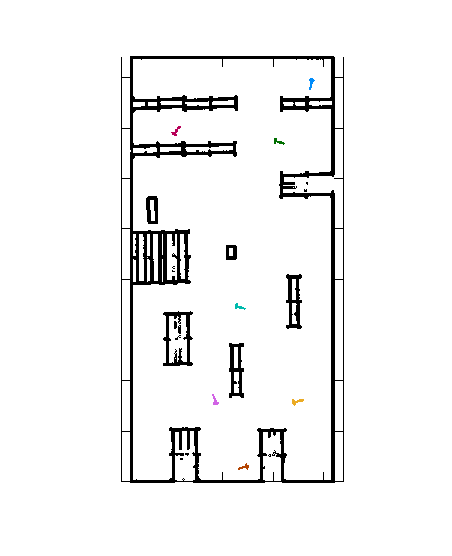
\includegraphics{./figures/parts/02/chapters/03/sections/04/map_warehouse}}%
    \gplfronttext
  \end{picture}%
\endgroup

    %\caption{\small Ο χάρτης $\bm{M}_W$ του περιβάλλοντος WAREHOUSE}
    \label{fig:02_03_04:map_warehouse}
  \end{subfigure}
  \begin{subfigure}{0.5\linewidth}
    % GNUPLOT: LaTeX picture with Postscript
\begingroup
  \makeatletter
  \providecommand\color[2][]{%
    \GenericError{(gnuplot) \space\space\space\@spaces}{%
      Package color not loaded in conjunction with
      terminal option `colourtext'%
    }{See the gnuplot documentation for explanation.%
    }{Either use 'blacktext' in gnuplot or load the package
      color.sty in LaTeX.}%
    \renewcommand\color[2][]{}%
  }%
  \providecommand\includegraphics[2][]{%
    \GenericError{(gnuplot) \space\space\space\@spaces}{%
      Package graphicx or graphics not loaded%
    }{See the gnuplot documentation for explanation.%
    }{The gnuplot epslatex terminal needs graphicx.sty or graphics.sty.}%
    \renewcommand\includegraphics[2][]{}%
  }%
  \providecommand\rotatebox[2]{#2}%
  \@ifundefined{ifGPcolor}{%
    \newif\ifGPcolor
    \GPcolorfalse
  }{}%
  \@ifundefined{ifGPblacktext}{%
    \newif\ifGPblacktext
    \GPblacktexttrue
  }{}%
  % define a \g@addto@macro without @ in the name:
  \let\gplgaddtomacro\g@addto@macro
  % define empty templates for all commands taking text:
  \gdef\gplfronttext{}%
  \gdef\gplfronttext{}%
  \makeatother
  \ifGPblacktext
    % no textcolor at all
    \def\colorrgb#1{}%
    \def\colorgray#1{}%
  \else
    % gray or color?
    \ifGPcolor
      \def\colorrgb#1{\color[rgb]{#1}}%
      \def\colorgray#1{\color[gray]{#1}}%
      \expandafter\def\csname LTw\endcsname{\color{white}}%
      \expandafter\def\csname LTb\endcsname{\color{black}}%
      \expandafter\def\csname LTa\endcsname{\color{black}}%
      \expandafter\def\csname LT0\endcsname{\color[rgb]{1,0,0}}%
      \expandafter\def\csname LT1\endcsname{\color[rgb]{0,1,0}}%
      \expandafter\def\csname LT2\endcsname{\color[rgb]{0,0,1}}%
      \expandafter\def\csname LT3\endcsname{\color[rgb]{1,0,1}}%
      \expandafter\def\csname LT4\endcsname{\color[rgb]{0,1,1}}%
      \expandafter\def\csname LT5\endcsname{\color[rgb]{1,1,0}}%
      \expandafter\def\csname LT6\endcsname{\color[rgb]{0,0,0}}%
      \expandafter\def\csname LT7\endcsname{\color[rgb]{1,0.3,0}}%
      \expandafter\def\csname LT8\endcsname{\color[rgb]{0.5,0.5,0.5}}%
    \else
      % gray
      \def\colorrgb#1{\color{black}}%
      \def\colorgray#1{\color[gray]{#1}}%
      \expandafter\def\csname LTw\endcsname{\color{white}}%
      \expandafter\def\csname LTb\endcsname{\color{black}}%
      \expandafter\def\csname LTa\endcsname{\color{black}}%
      \expandafter\def\csname LT0\endcsname{\color{black}}%
      \expandafter\def\csname LT1\endcsname{\color{black}}%
      \expandafter\def\csname LT2\endcsname{\color{black}}%
      \expandafter\def\csname LT3\endcsname{\color{black}}%
      \expandafter\def\csname LT4\endcsname{\color{black}}%
      \expandafter\def\csname LT5\endcsname{\color{black}}%
      \expandafter\def\csname LT6\endcsname{\color{black}}%
      \expandafter\def\csname LT7\endcsname{\color{black}}%
      \expandafter\def\csname LT8\endcsname{\color{black}}%
    \fi
  \fi
  \setlength{\unitlength}{0.0500bp}%
  \begin{picture}(4000.00,4000.00)%
    \gplgaddtomacro\gplfronttext{%
      \colorrgb{0.00,0.00,0.00}%
      \put(388,485){\makebox(0,0)[r]{\strut{}35}}%
      \colorrgb{0.00,0.00,0.00}%
      \put(388,829){\makebox(0,0)[r]{\strut{}40}}%
      \colorrgb{0.00,0.00,0.00}%
      \put(388,1174){\makebox(0,0)[r]{\strut{}45}}%
      \colorrgb{0.00,0.00,0.00}%
      \put(388,1518){\makebox(0,0)[r]{\strut{}50}}%
      \colorrgb{0.00,0.00,0.00}%
      \put(388,1862){\makebox(0,0)[r]{\strut{}55}}%
      \colorrgb{0.00,0.00,0.00}%
      \put(388,2207){\makebox(0,0)[r]{\strut{}60}}%
      \colorrgb{0.00,0.00,0.00}%
      \put(388,2551){\makebox(0,0)[r]{\strut{}65}}%
      \colorrgb{0.00,0.00,0.00}%
      \put(388,2895){\makebox(0,0)[r]{\strut{}70}}%
      \colorrgb{0.00,0.00,0.00}%
      \put(388,3240){\makebox(0,0)[r]{\strut{}75}}%
      \colorrgb{0.00,0.00,0.00}%
      \put(388,3584){\makebox(0,0)[r]{\strut{}80}}%
      \colorrgb{0.00,0.00,0.00}%
      \put(520,265){\makebox(0,0){\strut{}45}}%
      \colorrgb{0.00,0.00,0.00}%
      \put(864,265){\makebox(0,0){\strut{}50}}%
      \colorrgb{0.00,0.00,0.00}%
      \put(1209,265){\makebox(0,0){\strut{}55}}%
      \colorrgb{0.00,0.00,0.00}%
      \put(1553,265){\makebox(0,0){\strut{}60}}%
      \colorrgb{0.00,0.00,0.00}%
      \put(1897,265){\makebox(0,0){\strut{}65}}%
      \colorrgb{0.00,0.00,0.00}%
      \put(2242,265){\makebox(0,0){\strut{}70}}%
      \colorrgb{0.00,0.00,0.00}%
      \put(2586,265){\makebox(0,0){\strut{}75}}%
      \colorrgb{0.00,0.00,0.00}%
      \put(2930,265){\makebox(0,0){\strut{}80}}%
      \colorrgb{0.00,0.00,0.00}%
      \put(3275,265){\makebox(0,0){\strut{}85}}%
      \colorrgb{0.00,0.00,0.00}%
      \put(3619,265){\makebox(0,0){\strut{}90}}%
      \colorrgb{0.00,0.00,0.00}%
      \put(-118,2069){\rotatebox{90}{\makebox(0,0){\strut{}$y$ [m]}}}%
      \colorrgb{0.00,0.00,0.00}%
      \put(2069,-65){\makebox(0,0){\strut{}$x$ [m]}}%
    }%
    \gplgaddtomacro\gplfronttext{%
    }%
    \put(0,0){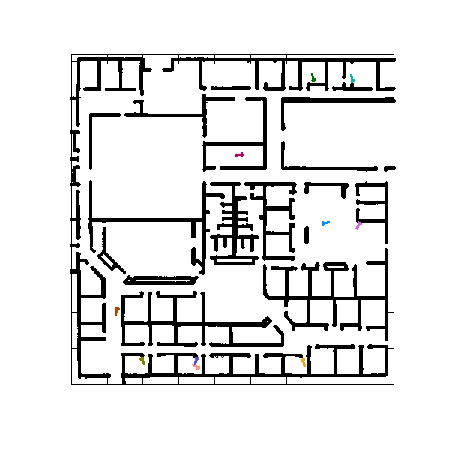
\includegraphics{./figures/parts/02/chapters/03/sections/04/map_willowgarage}}%
    \gplfronttext
  \end{picture}%
\endgroup

    %\caption{\small Ο χάρτης $\bm{M}_W$ του περιβάλλοντος WILLOWGARAGE}
    \label{fig:02_03_04:map_willowgarage}
  \end{subfigure}\\
  \begin{subfigure}{0.5\linewidth}
    \vspace{0.5cm}
    % GNUPLOT: LaTeX picture with Postscript
\begingroup
  \makeatletter
  \providecommand\color[2][]{%
    \GenericError{(gnuplot) \space\space\space\@spaces}{%
      Package color not loaded in conjunction with
      terminal option `colourtext'%
    }{See the gnuplot documentation for explanation.%
    }{Either use 'blacktext' in gnuplot or load the package
      color.sty in LaTeX.}%
    \renewcommand\color[2][]{}%
  }%
  \providecommand\includegraphics[2][]{%
    \GenericError{(gnuplot) \space\space\space\@spaces}{%
      Package graphicx or graphics not loaded%
    }{See the gnuplot documentation for explanation.%
    }{The gnuplot epslatex terminal needs graphicx.sty or graphics.sty.}%
    \renewcommand\includegraphics[2][]{}%
  }%
  \providecommand\rotatebox[2]{#2}%
  \@ifundefined{ifGPcolor}{%
    \newif\ifGPcolor
    \GPcolorfalse
  }{}%
  \@ifundefined{ifGPblacktext}{%
    \newif\ifGPblacktext
    \GPblacktexttrue
  }{}%
  % define a \g@addto@macro without @ in the name:
  \let\gplgaddtomacro\g@addto@macro
  % define empty templates for all commands taking text:
  \gdef\gplfronttext{}%
  \gdef\gplfronttext{}%
  \makeatother
  \ifGPblacktext
    % no textcolor at all
    \def\colorrgb#1{}%
    \def\colorgray#1{}%
  \else
    % gray or color?
    \ifGPcolor
      \def\colorrgb#1{\color[rgb]{#1}}%
      \def\colorgray#1{\color[gray]{#1}}%
      \expandafter\def\csname LTw\endcsname{\color{white}}%
      \expandafter\def\csname LTb\endcsname{\color{black}}%
      \expandafter\def\csname LTa\endcsname{\color{black}}%
      \expandafter\def\csname LT0\endcsname{\color[rgb]{1,0,0}}%
      \expandafter\def\csname LT1\endcsname{\color[rgb]{0,1,0}}%
      \expandafter\def\csname LT2\endcsname{\color[rgb]{0,0,1}}%
      \expandafter\def\csname LT3\endcsname{\color[rgb]{1,0,1}}%
      \expandafter\def\csname LT4\endcsname{\color[rgb]{0,1,1}}%
      \expandafter\def\csname LT5\endcsname{\color[rgb]{1,1,0}}%
      \expandafter\def\csname LT6\endcsname{\color[rgb]{0,0,0}}%
      \expandafter\def\csname LT7\endcsname{\color[rgb]{1,0.3,0}}%
      \expandafter\def\csname LT8\endcsname{\color[rgb]{0.5,0.5,0.5}}%
    \else
      % gray
      \def\colorrgb#1{\color{black}}%
      \def\colorgray#1{\color[gray]{#1}}%
      \expandafter\def\csname LTw\endcsname{\color{white}}%
      \expandafter\def\csname LTb\endcsname{\color{black}}%
      \expandafter\def\csname LTa\endcsname{\color{black}}%
      \expandafter\def\csname LT0\endcsname{\color{black}}%
      \expandafter\def\csname LT1\endcsname{\color{black}}%
      \expandafter\def\csname LT2\endcsname{\color{black}}%
      \expandafter\def\csname LT3\endcsname{\color{black}}%
      \expandafter\def\csname LT4\endcsname{\color{black}}%
      \expandafter\def\csname LT5\endcsname{\color{black}}%
      \expandafter\def\csname LT6\endcsname{\color{black}}%
      \expandafter\def\csname LT7\endcsname{\color{black}}%
      \expandafter\def\csname LT8\endcsname{\color{black}}%
    \fi
  \fi
  \setlength{\unitlength}{0.0500bp}%
  \begin{picture}(4000.00,4000.00)%
    \gplgaddtomacro\gplfronttext{%
      \colorrgb{0.00,0.00,0.00}%
      \put(388,1106){\makebox(0,0)[r]{\strut{}8}}%
      \colorrgb{0.00,0.00,0.00}%
      \put(388,1463){\makebox(0,0)[r]{\strut{}10}}%
      \colorrgb{0.00,0.00,0.00}%
      \put(388,1820){\makebox(0,0)[r]{\strut{}12}}%
      \colorrgb{0.00,0.00,0.00}%
      \put(388,2177){\makebox(0,0)[r]{\strut{}14}}%
      \colorrgb{0.00,0.00,0.00}%
      \put(388,2533){\makebox(0,0)[r]{\strut{}16}}%
      \colorrgb{0.00,0.00,0.00}%
      \put(388,2890){\makebox(0,0)[r]{\strut{}18}}%
      \colorrgb{0.00,0.00,0.00}%
      \put(388,3247){\makebox(0,0)[r]{\strut{}20}}%
      \colorrgb{0.00,0.00,0.00}%
      \put(527,610){\makebox(0,0){\strut{}4}}%
      \colorrgb{0.00,0.00,0.00}%
      \put(883,610){\makebox(0,0){\strut{}6}}%
      \colorrgb{0.00,0.00,0.00}%
      \put(1240,610){\makebox(0,0){\strut{}8}}%
      \colorrgb{0.00,0.00,0.00}%
      \put(1597,610){\makebox(0,0){\strut{}10}}%
      \colorrgb{0.00,0.00,0.00}%
      \put(1954,610){\makebox(0,0){\strut{}12}}%
      \colorrgb{0.00,0.00,0.00}%
      \put(2310,610){\makebox(0,0){\strut{}14}}%
      \colorrgb{0.00,0.00,0.00}%
      \put(2667,610){\makebox(0,0){\strut{}16}}%
      \colorrgb{0.00,0.00,0.00}%
      \put(3024,610){\makebox(0,0){\strut{}18}}%
      \colorrgb{0.00,0.00,0.00}%
      \put(3380,610){\makebox(0,0){\strut{}20}}%
      \colorrgb{0.00,0.00,0.00}%
      \put(-118,2069){\rotatebox{90}{\makebox(0,0){\strut{}$y$ [m]}}}%
      \colorrgb{0.00,0.00,0.00}%
      \put(2069,280){\makebox(0,0){\strut{}$x$ [m]}}%
      \put(2000,3600){\makebox(0,0){(ε') CSAL}}%
    }%
    \gplgaddtomacro\gplfronttext{%
    }%
    \put(0,0){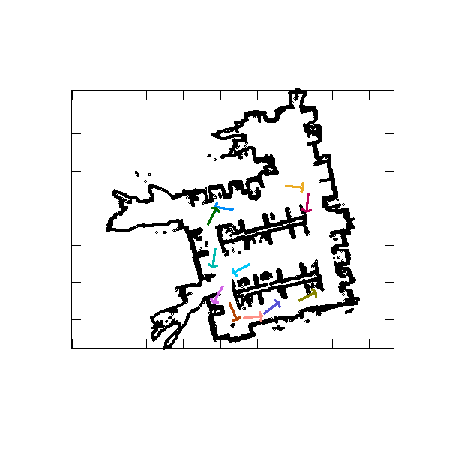
\includegraphics{./figures/parts/02/chapters/03/sections/04/map_csal}}%
    \gplfronttext
  \end{picture}%
\endgroup

    %\caption{\small Ο χάρτης $\bm{M}_A$ του περιβάλλοντος CSAL}
    \label{fig:02_03_04:map_csal}
  \end{subfigure}%
  \begin{subfigure}{0.5\linewidth}
    % GNUPLOT: LaTeX picture with Postscript
\begingroup
  \makeatletter
  \providecommand\color[2][]{%
    \GenericError{(gnuplot) \space\space\space\@spaces}{%
      Package color not loaded in conjunction with
      terminal option `colourtext'%
    }{See the gnuplot documentation for explanation.%
    }{Either use 'blacktext' in gnuplot or load the package
      color.sty in LaTeX.}%
    \renewcommand\color[2][]{}%
  }%
  \providecommand\includegraphics[2][]{%
    \GenericError{(gnuplot) \space\space\space\@spaces}{%
      Package graphicx or graphics not loaded%
    }{See the gnuplot documentation for explanation.%
    }{The gnuplot epslatex terminal needs graphicx.sty or graphics.sty.}%
    \renewcommand\includegraphics[2][]{}%
  }%
  \providecommand\rotatebox[2]{#2}%
  \@ifundefined{ifGPcolor}{%
    \newif\ifGPcolor
    \GPcolorfalse
  }{}%
  \@ifundefined{ifGPblacktext}{%
    \newif\ifGPblacktext
    \GPblacktexttrue
  }{}%
  % define a \g@addto@macro without @ in the name:
  \let\gplgaddtomacro\g@addto@macro
  % define empty templates for all commands taking text:
  \gdef\gplfronttext{}%
  \gdef\gplfronttext{}%
  \makeatother
  \ifGPblacktext
    % no textcolor at all
    \def\colorrgb#1{}%
    \def\colorgray#1{}%
  \else
    % gray or color?
    \ifGPcolor
      \def\colorrgb#1{\color[rgb]{#1}}%
      \def\colorgray#1{\color[gray]{#1}}%
      \expandafter\def\csname LTw\endcsname{\color{white}}%
      \expandafter\def\csname LTb\endcsname{\color{black}}%
      \expandafter\def\csname LTa\endcsname{\color{black}}%
      \expandafter\def\csname LT0\endcsname{\color[rgb]{1,0,0}}%
      \expandafter\def\csname LT1\endcsname{\color[rgb]{0,1,0}}%
      \expandafter\def\csname LT2\endcsname{\color[rgb]{0,0,1}}%
      \expandafter\def\csname LT3\endcsname{\color[rgb]{1,0,1}}%
      \expandafter\def\csname LT4\endcsname{\color[rgb]{0,1,1}}%
      \expandafter\def\csname LT5\endcsname{\color[rgb]{1,1,0}}%
      \expandafter\def\csname LT6\endcsname{\color[rgb]{0,0,0}}%
      \expandafter\def\csname LT7\endcsname{\color[rgb]{1,0.3,0}}%
      \expandafter\def\csname LT8\endcsname{\color[rgb]{0.5,0.5,0.5}}%
    \else
      % gray
      \def\colorrgb#1{\color{black}}%
      \def\colorgray#1{\color[gray]{#1}}%
      \expandafter\def\csname LTw\endcsname{\color{white}}%
      \expandafter\def\csname LTb\endcsname{\color{black}}%
      \expandafter\def\csname LTa\endcsname{\color{black}}%
      \expandafter\def\csname LT0\endcsname{\color{black}}%
      \expandafter\def\csname LT1\endcsname{\color{black}}%
      \expandafter\def\csname LT2\endcsname{\color{black}}%
      \expandafter\def\csname LT3\endcsname{\color{black}}%
      \expandafter\def\csname LT4\endcsname{\color{black}}%
      \expandafter\def\csname LT5\endcsname{\color{black}}%
      \expandafter\def\csname LT6\endcsname{\color{black}}%
      \expandafter\def\csname LT7\endcsname{\color{black}}%
      \expandafter\def\csname LT8\endcsname{\color{black}}%
    \fi
  \fi
  \setlength{\unitlength}{0.0500bp}%
  \begin{picture}(4000.00,4000.00)%
    \gplgaddtomacro\gplfronttext{%
      \colorrgb{0.00,0.00,0.00}%
      \put(1177,549){\makebox(0,0)[r]{\strut{}0}}%
      \colorrgb{0.00,0.00,0.00}%
      \put(1177,1092){\makebox(0,0)[r]{\strut{}5}}%
      \colorrgb{0.00,0.00,0.00}%
      \put(1177,1635){\makebox(0,0)[r]{\strut{}10}}%
      \colorrgb{0.00,0.00,0.00}%
      \put(1177,2178){\makebox(0,0)[r]{\strut{}15}}%
      \colorrgb{0.00,0.00,0.00}%
      \put(1177,2721){\makebox(0,0)[r]{\strut{}20}}%
      \colorrgb{0.00,0.00,0.00}%
      \put(1177,3264){\makebox(0,0)[r]{\strut{}25}}%
      \colorrgb{0.00,0.00,0.00}%
      \put(1418,220){\makebox(0,0){\strut{}0}}%
      \colorrgb{0.00,0.00,0.00}%
      \put(1635,220){\makebox(0,0){\strut{}2}}%
      \colorrgb{0.00,0.00,0.00}%
      \put(1852,220){\makebox(0,0){\strut{}4}}%
      \colorrgb{0.00,0.00,0.00}%
      \put(2069,220){\makebox(0,0){\strut{}6}}%
      \colorrgb{0.00,0.00,0.00}%
      \put(2286,220){\makebox(0,0){\strut{}8}}%
      \colorrgb{0.00,0.00,0.00}%
      \put(2503,220){\makebox(0,0){\strut{}10}}%
      \colorrgb{0.00,0.00,0.00}%
      \put(2790,220){\makebox(0,0){\strut{}12}}%
      \colorrgb{0.00,0.00,0.00}%
      \put(671,2069){\rotatebox{90}{\makebox(0,0){\strut{}$y$ [m]}}}%
      \colorrgb{0.00,0.00,0.00}%
      \put(2069,-110){\makebox(0,0){\strut{}$x$ [m]}}%
      \put(2100,3900){\makebox(0,0){(στ') LANDFILL}}%
    }%
    \gplgaddtomacro\gplfronttext{%
    }%
    \put(0,0){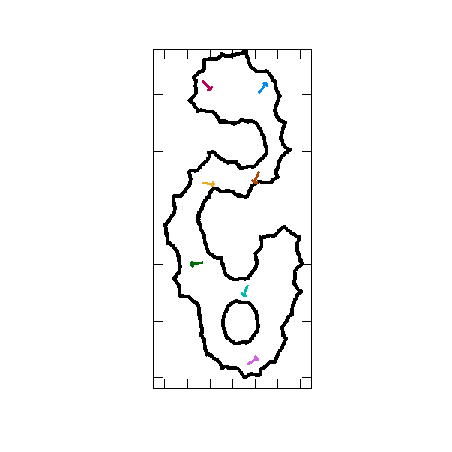
\includegraphics{./figures/parts/02/chapters/03/sections/04/map_dirtrack}}%
    \gplfronttext
  \end{picture}%
\endgroup

    %\caption{\small Ο χάρτης $\bm{M}_L$ του περιβάλλοντος LANDFILL}
    \label{fig:02_03_04:map_landfill}
  \end{subfigure}
\caption{\small Οι χάρτες των περιβαλλόντων στα οποία διενεργήθηκε η
         πειραματική διαδικασία}
\label{fig:02_03_04:maps_sim}
\end{figure}

Οι θέσεις στις οποίες τοποθετήθηκε το ρομπότ σε κάθε περιβάλλον καθορίστηκαν
από το σκοπό της αξιολόγησης του στόχου: στο περιβάλλον CORRIDOR το ρομπότ
τοποθετήθηκε κοντά στο ένα άκρο του ώστε να αξιολογηθεί η απόκριση των μεθόδων
σε συμμετρία του περιβάλλοντος, κοντά στη μέση ώστε να αξιολογηθεί η απόκρισή
τους σε σχέση με την ασάφεια του προσανατολισμού, και κοντά σε μια στροφή ώστε
να αξιολογηθεί η επίδραση της ανομοιομορφίας του περιβάλλοντος. Στο περιβάλλον
HOME το ρομπότ τοποθετήθηκε τυχαία και σε θέσεις που να αποτελούν προκλήσεις
για τις μεθόδους ευθυγράμμισης, κοντά ή μακριά από αντικείμενα, και σε θέσεις
των οποίων η γεωμετρία του περιβάλλοντος χώρου ήταν σχεδόν παρόμοια με αυτήν
άλλων μερών του περιβάλλοντος. Στο περιβάλλον WAREHOUSE τοποθετήθηκε σε
στάσεις τέτοιες που θα περίμενε κανείς ότι το ρομπότ θα εκκινούσε τη λειτουργία
του, και σε θέσεις τέτοιες που αποτελούν πρόκληση για την απόκριση των μεθόδων
ευθυγράμμισης λόγω έλλειψης χρήσιμων μετρήσεων (ένας τυπικός αισθητήρας LIDAR
αναφέρει ένδειξη μέγιστης εμβέλειας όταν η εν λόγω ακτίνα δεν συναντά
αντικείμενα στην πορεία της). Στο περιβάλλον WILLOWGARAGE το ρομπότ
τοποθετήθηκε σε δωμάτια που ήταν είτε πανομοιότυπα είτε σχεδόν πανομοιότυπα με
άλλα, και τυχαία. Ο προσανατολισμός της πραγματικής θέσης του ρομπότ δεν έχει
σημασία δεδομένου ότι ο αισθητήρας απόστασης είναι πανοραμικός, και καθορίστηκε
τυχαία μέσω δειγματοληψίας από μια ομοιόμορφη κατανομή $U(-\pi,\pi)$. Στον
πίνακα \ref{tbl:02_03_04:true_poses_simulation} παρατίθενται οι πραγματικές
στάσεις στις οποίες τοποθετήθηκε το ρομπότ σε κάθε προσομοιωμένο
περιβάλλον/χάρτη, μαζί με τους δείκτες τους και το χρώμα με το οποίο
σημειώνονται στοιχεία που αφορούν σε κάθε στάση στα επερχόμενα σχήματα.  Στον
πίνακα \ref{tbl:02_03_04:true_poses_experiment} παρατίθενται οι πραγματικές
στάσεις του ρομπότ στο περιβάλλον/χάρτη του CSAL. Λόγω της έλλειψης υποδομής
που θα μπορούσε να μετρήσει τη στάση του ρομπότ στο πραγματικό περιβάλλον CSAL
(π.χ.  ένα σύστημα MoCap), η στάση του ρομπότ εκτιμήθηκε με τη χρήση ενός
φίλτρου σωματιδίων (MCL) και ως εκ τούτου η εκτίμησή της μπορεί να υπόκειται σε
αναπόφευκτα σφάλματα εκτίμησης.

\begin{table}\centering
  \begin{tabular} {c|rrrc}                                                   \toprule
    Σημαίνον       & $x$ [m]   & $y$  [m]  & $\theta$ [rad]  &  Χρώμα     \\ \toprule
    \multicolumn{5}{c}{CORRIDOR}                                          \\ \midrule
    $\bm{p}_a^C$   & $11.56$   & $12.2$    & $-0.79$         & $\squarea$ \\
    $\bm{p}_b^C$   & $12.06$   & $8.2$     & $2.01$          & $\squareb$ \\
    $\bm{p}_c^C$   & $8.06$    & $9.20$    & $-3.28$         & $\squarec$ \\ \midrule
    \multicolumn{5}{c}{HOME}                                              \\ \midrule
    $\bm{p}_a^H$   & $14.44$   & $24.04$   & $0.065$         & $\squarea$ \\
    $\bm{p}_b^H$   & $17.84$   & $24.84$   & $1.33$          & $\squareb$ \\
    $\bm{p}_c^H$   & $15.0$    & $14.68$   & $0.68$          & $\squarec$ \\
    $\bm{p}_d^H$   & $22.0$    & $14.22$   & $-2.66$         & $\squared$ \\
    $\bm{p}_e^H$   & $26.0$    & $16.10$   & $0.69$          & $\squaree$ \\
    $\bm{p}_f^H$   & $24.46$   & $9.68$    & $-0.49$         & $\squaref$ \\
    $\bm{p}_g^H$   & $18.26$   & $11.02$   & $-3.10$         & $\squareg$ \\
    $\bm{p}_h^H$   & $27.64$   & $7.78$    & $-0.14$         & $\squareh$ \\
    $\bm{p}_i^H$   & $24.28$   & $21.44$   & $2.41$          & $\squarei$ \\
    $\bm{p}_j^H$   & $29.0$    & $28.64$   & $0.31$          & $\squarej$ \\
    $\bm{p}_k^H$   & $31.0$    & $12.2$    & $-2.19$         & $\squarek$ \\ \midrule
    \multicolumn{5}{c}{WAREHOUSE}                                         \\ \midrule
    $\bm{p}_a^W$   & $8.08$    & $3.02$    & $-2.85$         & $\squarea$ \\
    $\bm{p}_b^W$   & $35.16$   & $15.25$   & $-2.20$         & $\squareb$ \\
    $\bm{p}_c^W$   & $38.81$   & $2.35$    & $1.36$          & $\squarec$ \\
    $\bm{p}_d^W$   & $33.42$   & $4.92$    & $2.78$          & $\squared$ \\
    $\bm{p}_e^W$   & $17.08$   & $8.75$    & $2.83$          & $\squaree$ \\
    $\bm{p}_f^W$   & $8.63$    & $11.93$   & $-1.26$         & $\squaref$ \\
    $\bm{p}_g^W$   & $1.27$    & $9.5$     & $0.239$         & $\squareg$ \\ \midrule
    \multicolumn{5}{c}{WILLOWGARAGE}                                      \\ \midrule
    $\bm{p}_a^G$   & $77.56$   & $37.48$   & $-1.27$         & $\squarea$ \\
    $\bm{p}_b^G$   & $67.85$   & $66.90$   & $0.13$          & $\squareb$ \\
    $\bm{p}_c^G$   & $81.0$    & $57.60$   & $-2.97$         & $\squarec$ \\
    $\bm{p}_d^G$   & $78.55$   & $78.35$   & $-1.31$         & $\squared$ \\
    $\bm{p}_e^G$   & $84.0$    & $78.15$   & $0.94$          & $\squaree$ \\
    $\bm{p}_f^G$   & $84.75$   & $56.65$   & $1.02$          & $\squaref$ \\
    $\bm{p}_g^G$   & $51.15$   & $44.65$   & $1.29$          & $\squareg$ \\
    $\bm{p}_h^G$   & $61.95$   & $37.80$   & $-0.58$         & $\squareh$ \\
    $\bm{p}_i^G$   & $62.20$   & $37.76$   & $-1.22$         & $\squarei$ \\
    $\bm{p}_j^G$   & $55.20$   & $37.76$   & $0.91$          & $\squarej$ \\ \midrule
    \multicolumn{5}{c}{LANDFILL}                                          \\ \midrule
    $\bm{p}_a^L$   & $3.34$    & $17.19$   & $-0.082$        & $\squarea$ \\
    $\bm{p}_b^L$   & $3.34$    & $26.19$   & $-0.78$         & $\squareb$ \\
    $\bm{p}_c^L$   & $8.34$    & $25.19$   & $0.90$          & $\squarec$ \\
    $\bm{p}_d^L$   & $3.34$    & $10.19$   & $-2.97$         & $\squared$ \\
    $\bm{p}_e^L$   & $7.34$    & $8.19$    & $-1.93$         & $\squaree$ \\
    $\bm{p}_f^L$   & $7.34$    & $1.19$    & $0.58$          & $\squaref$ \\
    $\bm{p}_g^L$   & $8.34$    & $18.19$   & $-2.02$         & $\squareg$ \\ \bottomrule
  \end{tabular}
  \caption{\small Οι πραγματικές στάσης του ρομπότ στα πέντε προσομοιωμένα
           περιβάλλοντα και το χρώμα με το οποίο σημειώνονται στοιχεία για
           αυτές στα σχήματα}
  \label{tbl:02_03_04:true_poses_simulation}
\end{table}

\begin{table}[h]\centering
  \begin{tabular} {c|rrrc}                                                 \toprule
    Σημαίνον       & $x$ [m]   & $y$  [m]  & $\theta$ [rad]  & Χρώμα    \\ \toprule
    \multicolumn{4}{c}{CSAL AUTh}                                       \\ \midrule
    $\bm{p}_a^A$   & $15.47$   & $15.19$   & $-0.09$         & $\squarea$ \\
    $\bm{p}_b^A$   & $16.72$   & $14.81$   & $-1.67$         & $\squareb$ \\
    $\bm{p}_c^A$   & $12.67$   & $13.91$   & $2.98$          & $\squarec$ \\
    $\bm{p}_d^A$   & $11.30$   & $13.10$   & $1.08$          & $\squared$ \\
    $\bm{p}_e^A$   & $11.71$   & $11.83$   & $-1.70$         & $\squaree$ \\
    $\bm{p}_f^A$   & $12.12$   & $9.80$    & $-2.08$         & $\squaref$ \\
    $\bm{p}_g^A$   & $12.47$   & $8.89$    & $-1.14$         & $\squareg$ \\
    $\bm{p}_h^A$   & $13.22$   & $8.08$    & $0.10$          & $\squareh$ \\
    $\bm{p}_i^A$   & $14.32$   & $8.31$    & $0.65$          & $\squarei$ \\
    $\bm{p}_j^A$   & $16.22$   & $9.01$    & $0.47$          & $\squarej$ \\
    $\bm{p}_k^A$   & $13.56$   & $10.99$   & $-2.63$         & $\squarek$ \\ \bottomrule
  \end{tabular}
  \caption{\small Οι πραγματικές στάσης του ρομπότ στο πραγματικό περιβάλλον
           CSAL και το χρώμα με το οποίο σημειώνονται στοιχεία για αυτές στα
           σχήματα}
  \label{tbl:02_03_04:true_poses_experiment}
\end{table}


Δεδομένης της παρατήρησης \ref{remark:01_01_02_02:01}, μια λύση στάσης
θεωρείται ως ορθή όταν η απόκλιση της θέσης της από τη θέση της πραγματικής
στάσης είναι μικρότερη από $d_c = 1.0$ m.\footnote{Η τιμή της διακριτικής
απόστασης ανάμεσα σε έγκυρες και άκυρες λύσεις ορίστηκε ως τέτοια μετά από
πειράματα σε πραγματικές συνθήκες με το ίδιο ρομπότ, όπου χρησιμοποιήθηκε ο
αλγόριθμος Monte Carlo Localisation (MCL) για την παρακολούθηση της στάσης του.
Η μεθοδολογία ήταν η εξής: αρχικά το ρομπότ τοποθετήθηκε σε στάση σε δεδομένη
απόσταση από την πραγματική του θέση. Στη συνέχεια στο ρομπότ δόθηκε εντολή να
πλοηγηθεί αυτόνομα σε μία στάση στο χάρτη χρησιμοποιώντας την εκτίμηση της
στάσης του MCL ως πραγματική στάση του ρομπότ. Εάν αυτό δεν κατάφερε να
πλοηγηθεί στην καθορισμένη στάση τότε η απόσταση ανάμεσα στην θεωρούμενη ως
πραγματική του στάση και την πραγματική του στάση μειωνόταν έως ότου το ρομπότ
κατάφερε να πλοηγηθεί στην προκαθορισμένη στάση.}$^,$\footnote{Ως προς τον
προσανατολισμό δεν τέθηκε κάποιος περιορισμός, καθώς στην περίπτωση ορθής λύσης
ως προς τη θέση του ρομπότ δεν είναι βέβαιο ότι μία πιθανοτική μέθοδος
παρακολούθησης της στάσης του (η οποία χρησιμοποιείται στη συνέχεια της λύσης
του προβλήματος της εύρεσης της στάσης του βάσει καθολικής αβεβαιότητας) δεν
είναι σε θέση να μειώσει στο πέρασμα του χρόνου το σφάλμα προσανατολισμού καθώς
κινείται το ρομπότ. Σε κάθε περίπτωση, μετά την εύρεση της στάσης του ρομπότ
είναι δυνατόν να εκτελεστεί για μία τελική φορά ο αλγόριθμος ευθυγράμμισης για
την τελική εκτιμώμενη στάση, με αποτέλεσμα ακριβέστερη εκτίμηση στην περίπτωση
έγκυρης λύσης, και αδιάφορα εσφαλμένης εκτίμησης σε περίπτωση άκυρης λύσης (αν
η θέση είναι εσφαλμένη τότε δεν έχει σημασία ο προσανατολισμός της).} Όσες
λύσεις βρέθηκαν εκτός αυτής της ακτίνας ονομάζονται στο εξής άκυρες λύσεις.

Όσον αφορά στο μέγεθος του συνόλου $\mathcal{H}$ των υποθέσεων που
διασπείρονται σε κάθε περιβάλλον, σε συνέπεια με την παρατήρηση
\ref{appendix:remark:02_03_04:hypotheses_number}, καμία μέθοδος δεν στερήθηκε
υποθέσεων σε κανένα περιβάλλον: για τα περιβάλλοντα CORRIDOR, LANDFILL, και
CSAL $|\mathcal{H}_C| = |\mathcal{H}_L| = |\mathcal{H}_A| = 100$. Για τα
περιβάλλοντα περιβάλλοντα HOME και WAREHOUSE $|\mathcal{H}_H| = |\mathcal{H}_W|
= 200$, και για το περιβάλλον WILLOWGARAGE $|\mathcal{H}_G| = 500$.  Τα όρια
που αφορούν τον συντελεστή κλίμακας τέθηκαν σε $(\underline{\sigma},
\overline{\sigma}) = (0.9, 1.2)$. Το μήκος και το πλάτος των εικόνων που
εισάγονται στο FMI-SPOMF ορίστηκε σε $N_G = 2^8$: δοκιμές έδειξαν ότι αυτή η
ρύθμιση είναι το κατώτατο όριο ακριβούς διάκρισης μεταξύ αληθών και ψευδώς
θετικών λύσεων. Υψηλότερες τιμές του $N_G$ αυξάνουν την ευαισθησία της μεθόδου
όσον αφορά τη διάκριση μεταξύ θέσεων, αλλά με κόστος την αύξηση του χρόνου
εκτέλεσης. Ο αριθμός των επαναλήψεων του συστήματος εκτίμησης της θέσης του
FMIC και ο αριθμός των επαναλήψεων του PLICP ανά υπόθεση τέθηκαν σε $I = 10$.
Από τη ρύθμιση των τιμών των παραπάνω μεταβλητών σημειώνουμε ότι η προτεινόμενη
μέθοδος ευθυγράμμισης απαιτεί μικρότερο σύνολο μεταβλητών από αυτές του
PLICP (βλ. ενότητα \ref{subsection:02_02_05:02}), ικανοποιώντας την απαίτηση
(β) της πρώτης παραγράφου του κεφαλαίου.

Όλες οι προσομοιώσεις πραγματοποιήθηκαν στο περιβάλλον προσομοίωσης Gazebo,
μέσω \texttt{ROS}, σε \texttt{C++} και Ubuntu 16.04, με ένα επεξεργαστή δώδεκα
νημάτων, που λειτουργεί στα $4.00$ GHz, χρησιμοποιώντας έως και $32$ Gb μνήμης
RAM. Οι χάρτες των προσομοιωμένων περιβαλλόντων κατασκευάστηκαν χρησιμοποιώντας
το πακέτο χαρτογράφησης \texttt{slam\_karto} του
\texttt{ROS}.\footnote{\url{http://wiki.ros.org/slam\_karto}} Όλα τα πειράματα
πραγματοποιήθηκαν με έναν επεξεργαστή τεσσάρων νημάτων, με συχνότητα $2.30$
GHz, χρησιμοποιώντας έως και $8$ Gb μνήμης RAM. Ο χάρτης του περιβάλλοντος CSAL
κατασκευάστηκε με τη χρήση του πακέτου χαρτογράφησης \texttt{ROS}
\texttt{gmapping}.\footnote{\url{http://wiki.ros.org/gmapping}} Σημειώνουμε ότι
όσον αφορά στους χάρτες και τη χαρτογράφηση, το αποτέλεσμα του αλγορίθμου
χαρτογράφησης μπορεί να είναι ατελές με την έννοια ότι είναι δυνατή η εισαγωγή
ελεύθερου χώρου στη συνοχή ακόμη και ενός μεμονωμένου
εμποδίου.\footnote{Ατέλειες αυτού του τύπου οφείλονται στη διακριτή φύση του
αισθητήρα απόστασης όσον αφορά τη γωνιακή δειγματοληψία, στην ανάλυση του
χάρτη, και στο χρόνο εκτέλεσης του αλγορίθμου σε σύγκριση με τον όγκο των
πληροφοριών εισόδου.} Αυτό το είδος δομικού σφάλματος μπορεί να αλλοιώσει το
αποτέλεσμα της ευθυγράμμισής πραγματικών με εικονικές σαρώσεις, και ως εκ
τούτου πρέπει να δοθεί προσοχή ώστε είτε οι χάρτες να είναι ορθοί ως αποτέλεσμα
της χαρτογράφησης, ή να διορθώνεται ο λανθασμένα εισαχθέντας ελεύθερος
χώρος.\footnote{Έστω για παράδειγμα η περίπτωση όπου ένας τοίχος χωρίζει έναν
δωμάτιο από ένα άλλο. Στην περίπτωση ενός χάρτη πλέγματος η εισαγωγή του
ελεύθερου χώρου ως ``ρωγμή" στον τοίχο θα οδηγούσε σε μια κατάσταση όπου, εάν
μία εικονική σάρωση γίνεται σε απόσταση από τον τοίχο που βρίσκεται εντός του
μέγιστου εύρους του αισθητήρα, τουλάχιστον μία ακτίνα μπορεί να διαρρεύσει μέσα
από τη ρωγμή και να αναφέρει λανθασμένη μέτρηση απόστασης. Η συμπεριφορά αυτή
μπορεί να επιδεινωθεί εάν ο τοίχος αυτός διαχωρίζει τη χαρτογραφημένη περιοχή
από τη μη χαρτογραφημένη και η ρουτίνα εύρεσης τομών δεν έχει σχεδιαστεί για να
χειρίζεται μη χαρτογραφημένο χώρο.} Για την υλοποίηση του δισδιάστατου
μετασχηματισμού Fourier-Mellin χρησιμοποιήθηκε το σύστημα \texttt{imgreg\_dft}
γλώσσας \texttt{python}.\footnote{\url{https://pypi.org/project/imreg\_dft/}}
Όσον αφορά στις εισόδους του, αυτές ήταν δισδιάστατες εικόνες που παρήχθησαν
μέσω του \texttt{GNU Octave}
v.4.0.0:\footnote{\url{https://www.gnu.org/software/octave/}} οι πραγματικές
και εικονικές σαρώσεις απεικονίστηκαν σε μέγεθος πλέγματος $N_G \times N_G$
μέσω προβολής και διακριτοποίησης στο δισδιάστατο επίπεδο, και στη συνέχεια
γράφτηκαν στο δίσκο ως εικόνες μορφής \texttt{.png}. Εικόνες των μορφών
\texttt{.gif}, \texttt{.jpg}, και \texttt{.tiff} δεν παρήγαγαν επαρκή
αποτελέσματα.  Για την επεξεργασία μίας υπόθεσης στάσης ήταν απαραίτητη η
εισαγωγή χρονικής καθυστέρησης ανάμεσα σε αυτήν και την παραγωγή της εικόνας
που αφορά στο διάνυσμα εικονικών μετρήσεων που λήφθηκε από αυτήν, λόγω ανάγκης
αποθήκευσης της εικόνας στο δίσκο του υπολογιστή: οι χρόνοι εκτέλεσης του
PGL-FMIC στην ενότητα \ref{subsection:02_03_04:02} αντικατοπτρίζουν τους
ωφέλιμους χρόνους εκτέλεσης του αλγορίθμου ανά υπόθεση. Το υπολογιστικό κόστος
της προτεινόμενης μεθόδου είναι $483$ MB (συμπεριλαμβανομένων όλων των τμημάτων
λογισμικού) στη μνήμη, και περίπου $25\%$ σε χρήση ενός πυρήνα CPU.

Στις επόμενες ενότητες παρουσιάζονται τα αποτελέσματα των προσομοιώσεων και των
πειραμάτων που πραγματοποιήθηκαν με την προτεινόμενη μέθοδο (PGL-FMIC) και τον
αλγόριθμο PLICP για την επίλυση προβλήματος \ref{prob:02_03:the_problem} υπό
τις παραδοχές \ref{assumption:02_03_01:01} και \ref{assumption:02_03_01:02},
υπό συνθήκες ακινησίας του ρομπότ, στα παραπάνω έξι περιβάλλοντα, και υπό τις
συνθήκες που περιγράφηκαν σε αυτή την ενότητα.

%%%%%%%%%%%%%%%%%%%%%%%%%%%%%%%%%%%%%%%%%%%%%%%%%%%%%%%%%%%%%%%%%%%%%%%%%%%%%%%%
\subsection{Αποτελέσματα}
\label{subsection:02_03_04:02}

Στα ραβδογράμματα του σχήματος \ref{fig:02_03_04:outliers} απεικονίζονται τα
ποσοστά άκυρων λύσεων (εκτιμήσεων των οποίων η θέση έχει απόσταση από την
πραγματική θέση του ρομπότ άνω του $d_c = 1.0$ m) για τον PLICP και την
προτεινόμενη μέθοδο, για όλα τα περιβάλλοντα, στάσεις, και επίπεδα διαταραχών
μετρήσεων.

Τα διαγράμματα του σχήματος \ref{fig:02_03_04:sim_pose_errors_and_exec_times}
απεικονίζουν τη μέση τιμή σφάλματος στάσης για τους δύο αλγόριθμους
ανά περιβάλλον προσομοίωσης, στάση, και επίπεδο διαταραχών μετρήσεων
(αριστερά), και τους αντίστοιχους μέσους χρόνους εκτέλεσης (δεξιά). Η μονάδα
μέτρησης του σφάλματος στάσης είναι $(\text{m}^2 + \text{rad}^2)^{1/2}$ και
παραλείπεται στα διαγράμματα της ενότητας για λόγους ευαναγνωσιμότητας και
οικονομίας χώρου. Τα διαγράμματα του σχήματος
\ref{fig:02_03_04:csal_pose_errors_and_exec_times} απεικονίζουν τις ίδιες
μετρικές, αλλά όσο αφορά στα πειράματα στο πραγματικό περιβάλλον CSAL.
Τα σχήματα \ref{fig:appendix:03_04:sim_orientation_position_errors} και
\ref{fig:appendix:03_04:csal_orientation_position_errors} του παραρτήματος
\ref{appendix:03:location_and_orientation_errors} απεικονίζουν τα αντίστοιχα
μέσα σφάλματα προσανατολισμού και θέσης.

\begin{figure}
  \hspace{-1.5cm}
  % GNUPLOT: LaTeX picture with Postscript
\begingroup
  \makeatletter
  \providecommand\color[2][]{%
    \GenericError{(gnuplot) \space\space\space\@spaces}{%
      Package color not loaded in conjunction with
      terminal option `colourtext'%
    }{See the gnuplot documentation for explanation.%
    }{Either use 'blacktext' in gnuplot or load the package
      color.sty in LaTeX.}%
    \renewcommand\color[2][]{}%
  }%
  \providecommand\includegraphics[2][]{%
    \GenericError{(gnuplot) \space\space\space\@spaces}{%
      Package graphicx or graphics not loaded%
    }{See the gnuplot documentation for explanation.%
    }{The gnuplot epslatex terminal needs graphicx.sty or graphics.sty.}%
    \renewcommand\includegraphics[2][]{}%
  }%
  \providecommand\rotatebox[2]{#2}%
  \@ifundefined{ifGPcolor}{%
    \newif\ifGPcolor
    \GPcolorfalse
  }{}%
  \@ifundefined{ifGPblacktext}{%
    \newif\ifGPblacktext
    \GPblacktexttrue
  }{}%
  % define a \g@addto@macro without @ in the name:
  \let\gplgaddtomacro\g@addto@macro
  % define empty templates for all commands taking text:
  \gdef\gplfronttext{}%
  \gdef\gplfronttext{}%
  \makeatother
  \ifGPblacktext
    % no textcolor at all
    \def\colorrgb#1{}%
    \def\colorgray#1{}%
  \else
    % gray or color?
    \ifGPcolor
      \def\colorrgb#1{\color[rgb]{#1}}%
      \def\colorgray#1{\color[gray]{#1}}%
      \expandafter\def\csname LTw\endcsname{\color{white}}%
      \expandafter\def\csname LTb\endcsname{\color{black}}%
      \expandafter\def\csname LTa\endcsname{\color{black}}%
      \expandafter\def\csname LT0\endcsname{\color[rgb]{1,0,0}}%
      \expandafter\def\csname LT1\endcsname{\color[rgb]{0,1,0}}%
      \expandafter\def\csname LT2\endcsname{\color[rgb]{0,0,1}}%
      \expandafter\def\csname LT3\endcsname{\color[rgb]{1,0,1}}%
      \expandafter\def\csname LT4\endcsname{\color[rgb]{0,1,1}}%
      \expandafter\def\csname LT5\endcsname{\color[rgb]{1,1,0}}%
      \expandafter\def\csname LT6\endcsname{\color[rgb]{0,0,0}}%
      \expandafter\def\csname LT7\endcsname{\color[rgb]{1,0.3,0}}%
      \expandafter\def\csname LT8\endcsname{\color[rgb]{0.5,0.5,0.5}}%
    \else
      % gray
      \def\colorrgb#1{\color{black}}%
      \def\colorgray#1{\color[gray]{#1}}%
      \expandafter\def\csname LTw\endcsname{\color{white}}%
      \expandafter\def\csname LTb\endcsname{\color{black}}%
      \expandafter\def\csname LTa\endcsname{\color{black}}%
      \expandafter\def\csname LT0\endcsname{\color{black}}%
      \expandafter\def\csname LT1\endcsname{\color{black}}%
      \expandafter\def\csname LT2\endcsname{\color{black}}%
      \expandafter\def\csname LT3\endcsname{\color{black}}%
      \expandafter\def\csname LT4\endcsname{\color{black}}%
      \expandafter\def\csname LT5\endcsname{\color{black}}%
      \expandafter\def\csname LT6\endcsname{\color{black}}%
      \expandafter\def\csname LT7\endcsname{\color{black}}%
      \expandafter\def\csname LT8\endcsname{\color{black}}%
    \fi
  \fi
  \setlength{\unitlength}{0.0500bp}%
  \begin{picture}(11000.00,12000.00)%
    \gplgaddtomacro\gplfronttext{%
      \colorrgb{0.00,0.00,0.00}%
      \put(1431,10003){\makebox(0,0)[r]{\strut{}\small $0\%$}}%
      \colorrgb{0.00,0.00,0.00}%
      \put(1431,10277){\makebox(0,0)[r]{\strut{}\small $25\%$}}%
      \colorrgb{0.00,0.00,0.00}%
      \put(1431,10551){\makebox(0,0)[r]{\strut{}\small $50\%$}}%
      \colorrgb{0.00,0.00,0.00}%
      \put(1431,10825){\makebox(0,0)[r]{\strut{}\small $75\%$}}%
      \colorrgb{0.00,0.00,0.00}%
      \put(1431,11099){\makebox(0,0)[r]{\strut{}\small $100\%$}}%
      \colorrgb{0.00,0.00,0.00}%
      \put(2162,9783){\makebox(0,0){\strut{}\small $\bm{p}_a^C$}}%
      \colorrgb{0.00,0.00,0.00}%
      \put(3360,9783){\makebox(0,0){\strut{}\small $\bm{p}_b^C$}}%
      \colorrgb{0.00,0.00,0.00}%
      \put(4557,9783){\makebox(0,0){\strut{}\small $\bm{p}_c^C$}}%
      \colorrgb{0.00,0.00,0.00}%
      \put(465,10551){\rotatebox{90}{\makebox(0,0){\strut{}\small CORRIDOR}}}%
      \colorrgb{0.00,0.00,0.00}%
      \put(3359,11429){\makebox(0,0){\strut{}PLICP}}%
    }%
    \gplgaddtomacro\gplfronttext{%
    }%
    \gplgaddtomacro\gplfronttext{%
      \colorrgb{0.00,0.00,0.00}%
      \put(6096,10003){\makebox(0,0)[r]{\strut{}\small $0\%$}}%
      \colorrgb{0.00,0.00,0.00}%
      \put(6096,10277){\makebox(0,0)[r]{\strut{}\small $25\%$}}%
      \colorrgb{0.00,0.00,0.00}%
      \put(6096,10551){\makebox(0,0)[r]{\strut{}\small $50\%$}}%
      \colorrgb{0.00,0.00,0.00}%
      \put(6096,10825){\makebox(0,0)[r]{\strut{}\small $75\%$}}%
      \colorrgb{0.00,0.00,0.00}%
      \put(6096,11099){\makebox(0,0)[r]{\strut{}\small $100\%$}}%
      \colorrgb{0.00,0.00,0.00}%
      \put(6827,9783){\makebox(0,0){\strut{}\small $\bm{p}_a^C$}}%
      \colorrgb{0.00,0.00,0.00}%
      \put(8024,9783){\makebox(0,0){\strut{}\small $\bm{p}_b^C$}}%
      \colorrgb{0.00,0.00,0.00}%
      \put(9221,9783){\makebox(0,0){\strut{}\small $\bm{p}_c^C$}}%
      \colorrgb{0.00,0.00,0.00}%
      \put(8024,11429){\makebox(0,0){\strut{}PGL-FMIC}}%
    }%
    \gplgaddtomacro\gplfronttext{%
    }%
    \gplgaddtomacro\gplfronttext{%
      \colorrgb{0.00,0.00,0.00}%
      \put(1431,8266){\makebox(0,0)[r]{\strut{}\small $0\%$}}%
      \colorrgb{0.00,0.00,0.00}%
      \put(1431,8540){\makebox(0,0)[r]{\strut{}\small $25\%$}}%
      \colorrgb{0.00,0.00,0.00}%
      \put(1431,8814){\makebox(0,0)[r]{\strut{}\small $50\%$}}%
      \colorrgb{0.00,0.00,0.00}%
      \put(1431,9088){\makebox(0,0)[r]{\strut{}\small $75\%$}}%
      \colorrgb{0.00,0.00,0.00}%
      \put(1431,9362){\makebox(0,0)[r]{\strut{}\small $100\%$}}%
      \colorrgb{0.00,0.00,0.00}%
      \put(1726,8046){\makebox(0,0){\strut{}\small $\bm{p}_a^H$}}%
      \colorrgb{0.00,0.00,0.00}%
      \put(2053,8046){\makebox(0,0){\strut{}\small $\bm{p}_b^H$}}%
      \colorrgb{0.00,0.00,0.00}%
      \put(2380,8046){\makebox(0,0){\strut{}\small $\bm{p}_c^H$}}%
      \colorrgb{0.00,0.00,0.00}%
      \put(2706,8046){\makebox(0,0){\strut{}\small $\bm{p}_d^H$}}%
      \colorrgb{0.00,0.00,0.00}%
      \put(3033,8046){\makebox(0,0){\strut{}\small $\bm{p}_e^H$}}%
      \colorrgb{0.00,0.00,0.00}%
      \put(3360,8046){\makebox(0,0){\strut{}\small $\bm{p}_f^H$}}%
      \colorrgb{0.00,0.00,0.00}%
      \put(3686,8046){\makebox(0,0){\strut{}\small $\bm{p}_g^H$}}%
      \colorrgb{0.00,0.00,0.00}%
      \put(4013,8046){\makebox(0,0){\strut{}\small $\bm{p}_h^H$}}%
      \colorrgb{0.00,0.00,0.00}%
      \put(4339,8046){\makebox(0,0){\strut{}\small $\bm{p}_i^H$}}%
      \colorrgb{0.00,0.00,0.00}%
      \put(4666,8046){\makebox(0,0){\strut{}\small $\bm{p}_j^H$}}%
      \colorrgb{0.00,0.00,0.00}%
      \put(4993,8046){\makebox(0,0){\strut{}\small $\bm{p}_k^H$}}%
      \colorrgb{0.00,0.00,0.00}%
      \put(465,8814){\rotatebox{90}{\makebox(0,0){\strut{}\small HOME}}}%
    }%
    \gplgaddtomacro\gplfronttext{%
    }%
    \gplgaddtomacro\gplfronttext{%
      \colorrgb{0.00,0.00,0.00}%
      \put(6096,8266){\makebox(0,0)[r]{\strut{}\small $0\%$}}%
      \colorrgb{0.00,0.00,0.00}%
      \put(6096,8540){\makebox(0,0)[r]{\strut{}\small $25\%$}}%
      \colorrgb{0.00,0.00,0.00}%
      \put(6096,8814){\makebox(0,0)[r]{\strut{}\small $50\%$}}%
      \colorrgb{0.00,0.00,0.00}%
      \put(6096,9088){\makebox(0,0)[r]{\strut{}\small $75\%$}}%
      \colorrgb{0.00,0.00,0.00}%
      \put(6096,9362){\makebox(0,0)[r]{\strut{}\small $100\%$}}%
      \colorrgb{0.00,0.00,0.00}%
      \put(6391,8046){\makebox(0,0){\strut{}}}%
      \colorrgb{0.00,0.00,0.00}%
      \put(6718,8046){\makebox(0,0){\strut{}}}%
      \colorrgb{0.00,0.00,0.00}%
      \put(7044,8046){\makebox(0,0){\strut{}}}%
      \colorrgb{0.00,0.00,0.00}%
      \put(7371,8046){\makebox(0,0){\strut{}}}%
      \colorrgb{0.00,0.00,0.00}%
      \put(7697,8046){\makebox(0,0){\strut{}}}%
      \colorrgb{0.00,0.00,0.00}%
      \put(8024,8046){\makebox(0,0){\strut{}}}%
      \colorrgb{0.00,0.00,0.00}%
      \put(8351,8046){\makebox(0,0){\strut{}}}%
      \colorrgb{0.00,0.00,0.00}%
      \put(8677,8046){\makebox(0,0){\strut{}}}%
      \colorrgb{0.00,0.00,0.00}%
      \put(9004,8046){\makebox(0,0){\strut{}}}%
      \colorrgb{0.00,0.00,0.00}%
      \put(9330,8046){\makebox(0,0){\strut{}}}%
      \colorrgb{0.00,0.00,0.00}%
      \put(9657,8046){\makebox(0,0){\strut{}}}%
    }%
    \gplgaddtomacro\gplfronttext{%
    }%
    \gplgaddtomacro\gplfronttext{%
      \colorrgb{0.00,0.00,0.00}%
      \put(1431,6530){\makebox(0,0)[r]{\strut{}\small $0\%$}}%
      \colorrgb{0.00,0.00,0.00}%
      \put(1431,6804){\makebox(0,0)[r]{\strut{}\small $25\%$}}%
      \colorrgb{0.00,0.00,0.00}%
      \put(1431,7078){\makebox(0,0)[r]{\strut{}\small $50\%$}}%
      \colorrgb{0.00,0.00,0.00}%
      \put(1431,7352){\makebox(0,0)[r]{\strut{}\small $75\%$}}%
      \colorrgb{0.00,0.00,0.00}%
      \put(1431,7626){\makebox(0,0)[r]{\strut{}\small $100\%$}}%
      \colorrgb{0.00,0.00,0.00}%
      \put(1820,6310){\makebox(0,0){\strut{}\small $\bm{p}_a^W$}}%
      \colorrgb{0.00,0.00,0.00}%
      \put(2333,6310){\makebox(0,0){\strut{}\small $\bm{p}_b^W$}}%
      \colorrgb{0.00,0.00,0.00}%
      \put(2846,6310){\makebox(0,0){\strut{}\small $\bm{p}_c^W$}}%
      \colorrgb{0.00,0.00,0.00}%
      \put(3360,6310){\makebox(0,0){\strut{}\small $\bm{p}_d^W$}}%
      \colorrgb{0.00,0.00,0.00}%
      \put(3873,6310){\makebox(0,0){\strut{}\small $\bm{p}_e^W$}}%
      \colorrgb{0.00,0.00,0.00}%
      \put(4386,6310){\makebox(0,0){\strut{}\small $\bm{p}_f^W$}}%
      \colorrgb{0.00,0.00,0.00}%
      \put(4899,6310){\makebox(0,0){\strut{}\small $\bm{p}_g^W$}}%
      \colorrgb{0.00,0.00,0.00}%
      \put(465,7078){\rotatebox{90}{\makebox(0,0){\strut{}\small WAREHOUSE}}}%
    }%
    \gplgaddtomacro\gplfronttext{%
    }%
    \gplgaddtomacro\gplfronttext{%
      \colorrgb{0.00,0.00,0.00}%
      \put(6096,6530){\makebox(0,0)[r]{\strut{}\small $0\%$}}%
      \colorrgb{0.00,0.00,0.00}%
      \put(6096,6804){\makebox(0,0)[r]{\strut{}\small $25\%$}}%
      \colorrgb{0.00,0.00,0.00}%
      \put(6096,7078){\makebox(0,0)[r]{\strut{}\small $50\%$}}%
      \colorrgb{0.00,0.00,0.00}%
      \put(6096,7352){\makebox(0,0)[r]{\strut{}\small $75\%$}}%
      \colorrgb{0.00,0.00,0.00}%
      \put(6096,7626){\makebox(0,0)[r]{\strut{}\small $100\%$}}%
      \colorrgb{0.00,0.00,0.00}%
      \put(6485,6310){\makebox(0,0){\strut{}\small $\bm{p}_a^W$}}%
      \colorrgb{0.00,0.00,0.00}%
      \put(6998,6310){\makebox(0,0){\strut{}\small $\bm{p}_b^W$}}%
      \colorrgb{0.00,0.00,0.00}%
      \put(7511,6310){\makebox(0,0){\strut{}\small $\bm{p}_c^W$}}%
      \colorrgb{0.00,0.00,0.00}%
      \put(8024,6310){\makebox(0,0){\strut{}\small $\bm{p}_d^W$}}%
      \colorrgb{0.00,0.00,0.00}%
      \put(8537,6310){\makebox(0,0){\strut{}\small $\bm{p}_e^W$}}%
      \colorrgb{0.00,0.00,0.00}%
      \put(9050,6310){\makebox(0,0){\strut{}\small $\bm{p}_f^W$}}%
      \colorrgb{0.00,0.00,0.00}%
      \put(9563,6310){\makebox(0,0){\strut{}\small $\bm{p}_g^W$}}%
    }%
    \gplgaddtomacro\gplfronttext{%
    }%
    \gplgaddtomacro\gplfronttext{%
      \colorrgb{0.00,0.00,0.00}%
      \put(1431,4793){\makebox(0,0)[r]{\strut{}\small $0\%$}}%
      \colorrgb{0.00,0.00,0.00}%
      \put(1431,5067){\makebox(0,0)[r]{\strut{}\small $25\%$}}%
      \colorrgb{0.00,0.00,0.00}%
      \put(1431,5341){\makebox(0,0)[r]{\strut{}\small $50\%$}}%
      \colorrgb{0.00,0.00,0.00}%
      \put(1431,5615){\makebox(0,0)[r]{\strut{}\small $75\%$}}%
      \colorrgb{0.00,0.00,0.00}%
      \put(1431,5889){\makebox(0,0)[r]{\strut{}\small $100\%$}}%
      \colorrgb{0.00,0.00,0.00}%
      \put(1743,4573){\makebox(0,0){\strut{}\small $\bm{p}_a^G$}}%
      \colorrgb{0.00,0.00,0.00}%
      \put(2102,4573){\makebox(0,0){\strut{}\small $\bm{p}_b^G$}}%
      \colorrgb{0.00,0.00,0.00}%
      \put(2461,4573){\makebox(0,0){\strut{}\small $\bm{p}_c^G$}}%
      \colorrgb{0.00,0.00,0.00}%
      \put(2821,4573){\makebox(0,0){\strut{}\small $\bm{p}_d^G$}}%
      \colorrgb{0.00,0.00,0.00}%
      \put(3180,4573){\makebox(0,0){\strut{}\small $\bm{p}_e^G$}}%
      \colorrgb{0.00,0.00,0.00}%
      \put(3539,4573){\makebox(0,0){\strut{}\small $\bm{p}_f^G$}}%
      \colorrgb{0.00,0.00,0.00}%
      \put(3898,4573){\makebox(0,0){\strut{}\small $\bm{p}_g^G$}}%
      \colorrgb{0.00,0.00,0.00}%
      \put(4258,4573){\makebox(0,0){\strut{}\small $\bm{p}_h^G$}}%
      \colorrgb{0.00,0.00,0.00}%
      \put(4617,4573){\makebox(0,0){\strut{}\small $\bm{p}_i^G$}}%
      \colorrgb{0.00,0.00,0.00}%
      \put(4976,4573){\makebox(0,0){\strut{}\small $\bm{p}_j^G$}}%
      \colorrgb{0.00,0.00,0.00}%
      \put(465,5341){\rotatebox{90}{\makebox(0,0){\strut{}\small WILLOWGARAGE}}}%
    }%
    \gplgaddtomacro\gplfronttext{%
    }%
    \gplgaddtomacro\gplfronttext{%
      \colorrgb{0.00,0.00,0.00}%
      \put(6096,4793){\makebox(0,0)[r]{\strut{}\small $0\%$}}%
      \colorrgb{0.00,0.00,0.00}%
      \put(6096,5067){\makebox(0,0)[r]{\strut{}\small $25\%$}}%
      \colorrgb{0.00,0.00,0.00}%
      \put(6096,5341){\makebox(0,0)[r]{\strut{}\small $50\%$}}%
      \colorrgb{0.00,0.00,0.00}%
      \put(6096,5615){\makebox(0,0)[r]{\strut{}\small $75\%$}}%
      \colorrgb{0.00,0.00,0.00}%
      \put(6096,5889){\makebox(0,0)[r]{\strut{}\small $100\%$}}%
      \colorrgb{0.00,0.00,0.00}%
      \put(6408,4573){\makebox(0,0){\strut{}\small $\bm{p}_a^G$}}%
      \colorrgb{0.00,0.00,0.00}%
      \put(6767,4573){\makebox(0,0){\strut{}\small $\bm{p}_b^G$}}%
      \colorrgb{0.00,0.00,0.00}%
      \put(7126,4573){\makebox(0,0){\strut{}\small $\bm{p}_c^G$}}%
      \colorrgb{0.00,0.00,0.00}%
      \put(7485,4573){\makebox(0,0){\strut{}\small $\bm{p}_d^G$}}%
      \colorrgb{0.00,0.00,0.00}%
      \put(7844,4573){\makebox(0,0){\strut{}\small $\bm{p}_e^G$}}%
      \colorrgb{0.00,0.00,0.00}%
      \put(8204,4573){\makebox(0,0){\strut{}\small $\bm{p}_f^G$}}%
      \colorrgb{0.00,0.00,0.00}%
      \put(8563,4573){\makebox(0,0){\strut{}\small $\bm{p}_g^G$}}%
      \colorrgb{0.00,0.00,0.00}%
      \put(8922,4573){\makebox(0,0){\strut{}\small $\bm{p}_h^G$}}%
      \colorrgb{0.00,0.00,0.00}%
      \put(9281,4573){\makebox(0,0){\strut{}\small $\bm{p}_i^G$}}%
      \colorrgb{0.00,0.00,0.00}%
      \put(9640,4573){\makebox(0,0){\strut{}\small $\bm{p}_j^G$}}%
    }%
    \gplgaddtomacro\gplfronttext{%
    }%
    \gplgaddtomacro\gplfronttext{%
      \colorrgb{0.00,0.00,0.00}%
      \put(1431,3056){\makebox(0,0)[r]{\strut{}\small $0\%$}}%
      \colorrgb{0.00,0.00,0.00}%
      \put(1431,3330){\makebox(0,0)[r]{\strut{}\small $25\%$}}%
      \colorrgb{0.00,0.00,0.00}%
      \put(1431,3604){\makebox(0,0)[r]{\strut{}\small $50\%$}}%
      \colorrgb{0.00,0.00,0.00}%
      \put(1431,3878){\makebox(0,0)[r]{\strut{}\small $75\%$}}%
      \colorrgb{0.00,0.00,0.00}%
      \put(1431,4152){\makebox(0,0)[r]{\strut{}\small $100\%$}}%
      \colorrgb{0.00,0.00,0.00}%
      \put(1820,2836){\makebox(0,0){\strut{}\small $\bm{p}_a^L$}}%
      \colorrgb{0.00,0.00,0.00}%
      \put(2333,2836){\makebox(0,0){\strut{}\small $\bm{p}_b^L$}}%
      \colorrgb{0.00,0.00,0.00}%
      \put(2846,2836){\makebox(0,0){\strut{}\small $\bm{p}_c^L$}}%
      \colorrgb{0.00,0.00,0.00}%
      \put(3360,2836){\makebox(0,0){\strut{}\small $\bm{p}_d^L$}}%
      \colorrgb{0.00,0.00,0.00}%
      \put(3873,2836){\makebox(0,0){\strut{}\small $\bm{p}_e^L$}}%
      \colorrgb{0.00,0.00,0.00}%
      \put(4386,2836){\makebox(0,0){\strut{}\small $\bm{p}_f^L$}}%
      \colorrgb{0.00,0.00,0.00}%
      \put(4899,2836){\makebox(0,0){\strut{}\small $\bm{p}_g^L$}}%
      \colorrgb{0.00,0.00,0.00}%
      \put(465,3604){\rotatebox{90}{\makebox(0,0){\strut{}\small LANDFILL}}}%
    }%
    \gplgaddtomacro\gplfronttext{%
    }%
    \gplgaddtomacro\gplfronttext{%
      \colorrgb{0.00,0.00,0.00}%
      \put(6096,3056){\makebox(0,0)[r]{\strut{}\small $0\%$}}%
      \colorrgb{0.00,0.00,0.00}%
      \put(6096,3330){\makebox(0,0)[r]{\strut{}\small $25\%$}}%
      \colorrgb{0.00,0.00,0.00}%
      \put(6096,3604){\makebox(0,0)[r]{\strut{}\small $50\%$}}%
      \colorrgb{0.00,0.00,0.00}%
      \put(6096,3878){\makebox(0,0)[r]{\strut{}\small $75\%$}}%
      \colorrgb{0.00,0.00,0.00}%
      \put(6096,4152){\makebox(0,0)[r]{\strut{}\small $100\%$}}%
      \colorrgb{0.00,0.00,0.00}%
      \put(6485,2836){\makebox(0,0){\strut{}\small $\bm{p}_a^L$}}%
      \colorrgb{0.00,0.00,0.00}%
      \put(6998,2836){\makebox(0,0){\strut{}\small $\bm{p}_b^L$}}%
      \colorrgb{0.00,0.00,0.00}%
      \put(7511,2836){\makebox(0,0){\strut{}\small $\bm{p}_c^L$}}%
      \colorrgb{0.00,0.00,0.00}%
      \put(8024,2836){\makebox(0,0){\strut{}\small $\bm{p}_d^L$}}%
      \colorrgb{0.00,0.00,0.00}%
      \put(8537,2836){\makebox(0,0){\strut{}\small $\bm{p}_e^L$}}%
      \colorrgb{0.00,0.00,0.00}%
      \put(9050,2836){\makebox(0,0){\strut{}\small $\bm{p}_f^L$}}%
      \colorrgb{0.00,0.00,0.00}%
      \put(9563,2836){\makebox(0,0){\strut{}\small $\bm{p}_g^L$}}%
    }%
    \gplgaddtomacro\gplfronttext{%
    }%
    \gplgaddtomacro\gplfronttext{%
      \colorrgb{0.00,0.00,0.00}%
      \put(1431,1320){\makebox(0,0)[r]{\strut{}\small $0\%$}}%
      \colorrgb{0.00,0.00,0.00}%
      \put(1431,1539){\makebox(0,0)[r]{\strut{}\small $20\%$}}%
      \colorrgb{0.00,0.00,0.00}%
      \put(1431,1758){\makebox(0,0)[r]{\strut{}\small $40\%$}}%
      \colorrgb{0.00,0.00,0.00}%
      \put(1431,1978){\makebox(0,0)[r]{\strut{}\small $60\%$}}%
      \colorrgb{0.00,0.00,0.00}%
      \put(1431,2197){\makebox(0,0)[r]{\strut{}\small $80\%$}}%
      \colorrgb{0.00,0.00,0.00}%
      \put(1431,2416){\makebox(0,0)[r]{\strut{}\small $100\%$}}%
      \colorrgb{0.00,0.00,0.00}%
      \put(1726,1100){\makebox(0,0){\strut{}\small $\bm{p}_a^A$}}%
      \colorrgb{0.00,0.00,0.00}%
      \put(2053,1100){\makebox(0,0){\strut{}\small $\bm{p}_b^A$}}%
      \colorrgb{0.00,0.00,0.00}%
      \put(2380,1100){\makebox(0,0){\strut{}\small $\bm{p}_c^A$}}%
      \colorrgb{0.00,0.00,0.00}%
      \put(2706,1100){\makebox(0,0){\strut{}\small $\bm{p}_d^A$}}%
      \colorrgb{0.00,0.00,0.00}%
      \put(3033,1100){\makebox(0,0){\strut{}\small $\bm{p}_e^A$}}%
      \colorrgb{0.00,0.00,0.00}%
      \put(3360,1100){\makebox(0,0){\strut{}\small $\bm{p}_f^A$}}%
      \colorrgb{0.00,0.00,0.00}%
      \put(3686,1100){\makebox(0,0){\strut{}\small $\bm{p}_g^A$}}%
      \colorrgb{0.00,0.00,0.00}%
      \put(4013,1100){\makebox(0,0){\strut{}\small $\bm{p}_h^A$}}%
      \colorrgb{0.00,0.00,0.00}%
      \put(4339,1100){\makebox(0,0){\strut{}\small $\bm{p}_i^A$}}%
      \colorrgb{0.00,0.00,0.00}%
      \put(4666,1100){\makebox(0,0){\strut{}\small $\bm{p}_j^A$}}%
      \colorrgb{0.00,0.00,0.00}%
      \put(4993,1100){\makebox(0,0){\strut{}\small $\bm{p}_k^A$}}%
      \colorrgb{0.00,0.00,0.00}%
      \put(465,1868){\rotatebox{90}{\makebox(0,0){\strut{}\small CSAL}}}%
      \colorrgb{0.00,0.00,0.00}%
      \put(3359,770){\makebox(0,0){\strut{}Σημαίνον στάσης}}%
    }%
    \gplgaddtomacro\gplfronttext{%
    }%
    \gplgaddtomacro\gplfronttext{%
      \colorrgb{0.00,0.00,0.00}%
      \put(6096,1320){\makebox(0,0)[r]{\strut{}\small $0\%$}}%
      \colorrgb{0.00,0.00,0.00}%
      \put(6096,1539){\makebox(0,0)[r]{\strut{}\small $20\%$}}%
      \colorrgb{0.00,0.00,0.00}%
      \put(6096,1758){\makebox(0,0)[r]{\strut{}\small $40\%$}}%
      \colorrgb{0.00,0.00,0.00}%
      \put(6096,1978){\makebox(0,0)[r]{\strut{}\small $60\%$}}%
      \colorrgb{0.00,0.00,0.00}%
      \put(6096,2197){\makebox(0,0)[r]{\strut{}\small $80\%$}}%
      \colorrgb{0.00,0.00,0.00}%
      \put(6096,2416){\makebox(0,0)[r]{\strut{}\small $100\%$}}%
      \colorrgb{0.00,0.00,0.00}%
      \put(6391,1100){\makebox(0,0){\strut{}\small $\bm{p}_a^A$}}%
      \colorrgb{0.00,0.00,0.00}%
      \put(6718,1100){\makebox(0,0){\strut{}\small $\bm{p}_b^A$}}%
      \colorrgb{0.00,0.00,0.00}%
      \put(7044,1100){\makebox(0,0){\strut{}\small $\bm{p}_c^A$}}%
      \colorrgb{0.00,0.00,0.00}%
      \put(7371,1100){\makebox(0,0){\strut{}\small $\bm{p}_d^A$}}%
      \colorrgb{0.00,0.00,0.00}%
      \put(7697,1100){\makebox(0,0){\strut{}\small $\bm{p}_e^A$}}%
      \colorrgb{0.00,0.00,0.00}%
      \put(8024,1100){\makebox(0,0){\strut{}\small $\bm{p}_f^A$}}%
      \colorrgb{0.00,0.00,0.00}%
      \put(8351,1100){\makebox(0,0){\strut{}\small $\bm{p}_g^A$}}%
      \colorrgb{0.00,0.00,0.00}%
      \put(8677,1100){\makebox(0,0){\strut{}\small $\bm{p}_h^A$}}%
      \colorrgb{0.00,0.00,0.00}%
      \put(9004,1100){\makebox(0,0){\strut{}\small $\bm{p}_i^A$}}%
      \colorrgb{0.00,0.00,0.00}%
      \put(9330,1100){\makebox(0,0){\strut{}\small $\bm{p}_j^A$}}%
      \colorrgb{0.00,0.00,0.00}%
      \put(9657,1100){\makebox(0,0){\strut{}\small $\bm{p}_k^A$}}%
    }%
    \gplgaddtomacro\gplfronttext{%
    }%
    \put(0,0){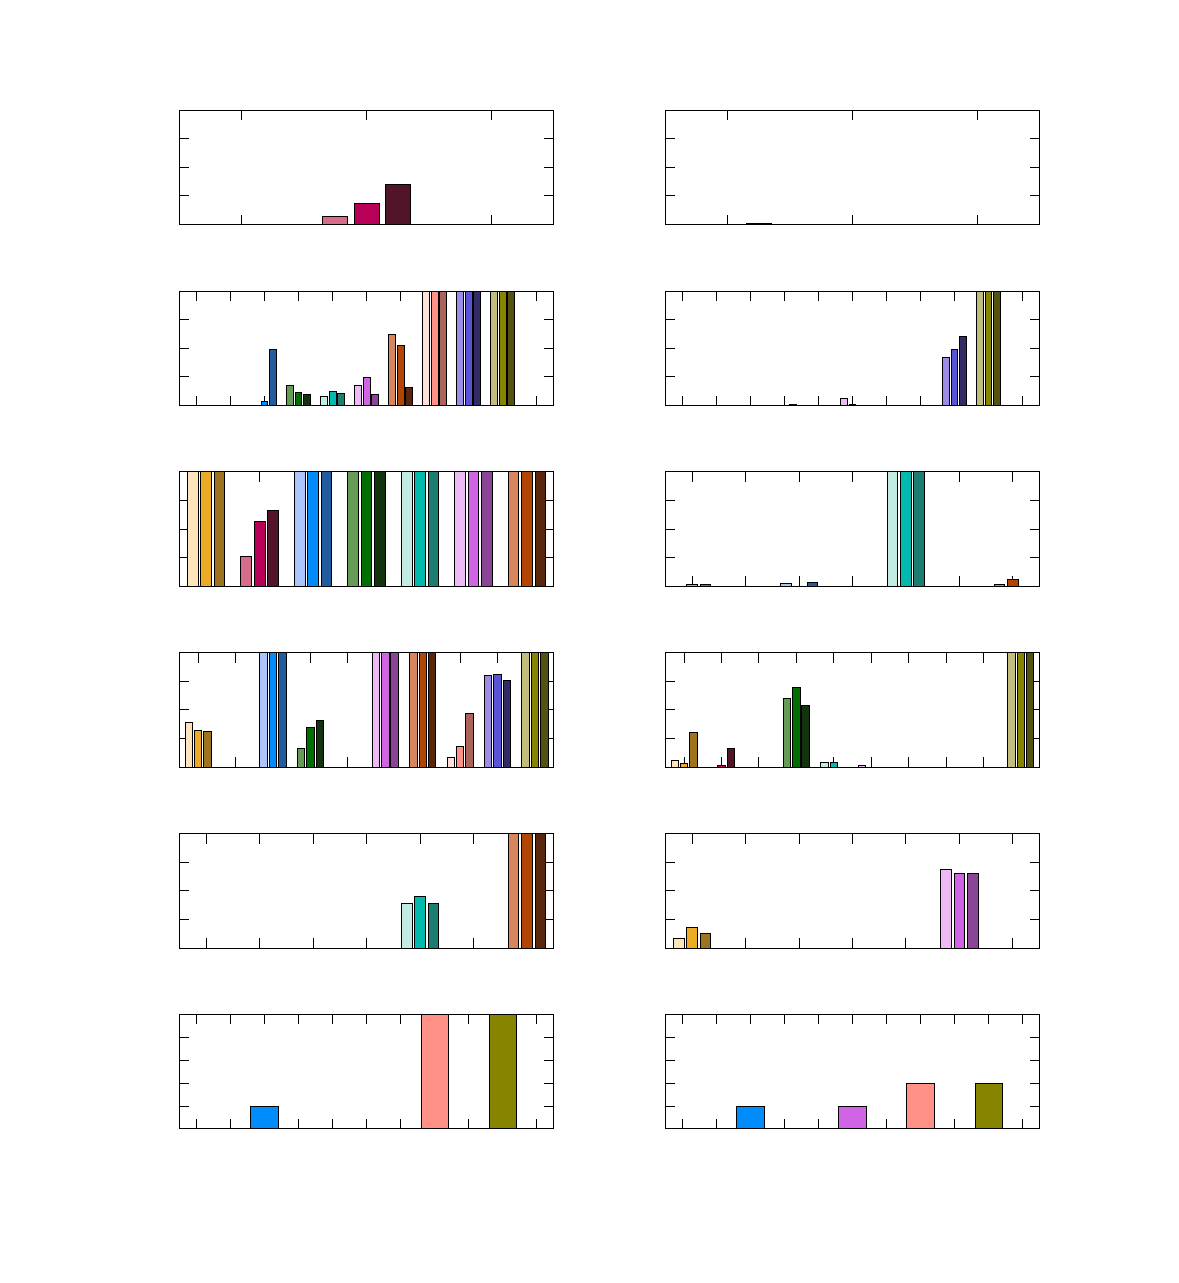
\includegraphics{./figures/parts/02/chapters/03/sections/04/outliers}}%
    \gplfronttext
  \end{picture}%
\endgroup

  \vspace{-1cm}
\caption{\small Ποσοστά άκυρων λύσεων ανά αλγόριθμο, περιβάλλον ελέγχου,
         πραγματική στάση του ρομπότ, και επίπεδο διαταραχών μετρήσεων του
         αισθητήρα αποστάσεων. Κάθε τριάδα ράβδων απεικονίζει τα ποσοστά
         άκυρων λύσεων για κανονικά κατανεμημένο θόρυβο μέτρησης, μηδενικής
         μέσης τιμής, και τυπικής απόκλισης $\sigma = 0.01, 0.02, 0.05$ m}
\label{fig:02_03_04:outliers}
\end{figure}

\begin{figure}
  \hspace{-0.5cm}
  \begin{subfigure}{0.5\linewidth}
    % GNUPLOT: LaTeX picture with Postscript
\begingroup
  \makeatletter
  \providecommand\color[2][]{%
    \GenericError{(gnuplot) \space\space\space\@spaces}{%
      Package color not loaded in conjunction with
      terminal option `colourtext'%
    }{See the gnuplot documentation for explanation.%
    }{Either use 'blacktext' in gnuplot or load the package
      color.sty in LaTeX.}%
    \renewcommand\color[2][]{}%
  }%
  \providecommand\includegraphics[2][]{%
    \GenericError{(gnuplot) \space\space\space\@spaces}{%
      Package graphicx or graphics not loaded%
    }{See the gnuplot documentation for explanation.%
    }{The gnuplot epslatex terminal needs graphicx.sty or graphics.sty.}%
    \renewcommand\includegraphics[2][]{}%
  }%
  \providecommand\rotatebox[2]{#2}%
  \@ifundefined{ifGPcolor}{%
    \newif\ifGPcolor
    \GPcolorfalse
  }{}%
  \@ifundefined{ifGPblacktext}{%
    \newif\ifGPblacktext
    \GPblacktexttrue
  }{}%
  % define a \g@addto@macro without @ in the name:
  \let\gplgaddtomacro\g@addto@macro
  % define empty templates for all commands taking text:
  \gdef\gplfronttext{}%
  \gdef\gplfronttext{}%
  \makeatother
  \ifGPblacktext
    % no textcolor at all
    \def\colorrgb#1{}%
    \def\colorgray#1{}%
  \else
    % gray or color?
    \ifGPcolor
      \def\colorrgb#1{\color[rgb]{#1}}%
      \def\colorgray#1{\color[gray]{#1}}%
      \expandafter\def\csname LTw\endcsname{\color{white}}%
      \expandafter\def\csname LTb\endcsname{\color{black}}%
      \expandafter\def\csname LTa\endcsname{\color{black}}%
      \expandafter\def\csname LT0\endcsname{\color[rgb]{1,0,0}}%
      \expandafter\def\csname LT1\endcsname{\color[rgb]{0,1,0}}%
      \expandafter\def\csname LT2\endcsname{\color[rgb]{0,0,1}}%
      \expandafter\def\csname LT3\endcsname{\color[rgb]{1,0,1}}%
      \expandafter\def\csname LT4\endcsname{\color[rgb]{0,1,1}}%
      \expandafter\def\csname LT5\endcsname{\color[rgb]{1,1,0}}%
      \expandafter\def\csname LT6\endcsname{\color[rgb]{0,0,0}}%
      \expandafter\def\csname LT7\endcsname{\color[rgb]{1,0.3,0}}%
      \expandafter\def\csname LT8\endcsname{\color[rgb]{0.5,0.5,0.5}}%
    \else
      % gray
      \def\colorrgb#1{\color{black}}%
      \def\colorgray#1{\color[gray]{#1}}%
      \expandafter\def\csname LTw\endcsname{\color{white}}%
      \expandafter\def\csname LTb\endcsname{\color{black}}%
      \expandafter\def\csname LTa\endcsname{\color{black}}%
      \expandafter\def\csname LT0\endcsname{\color{black}}%
      \expandafter\def\csname LT1\endcsname{\color{black}}%
      \expandafter\def\csname LT2\endcsname{\color{black}}%
      \expandafter\def\csname LT3\endcsname{\color{black}}%
      \expandafter\def\csname LT4\endcsname{\color{black}}%
      \expandafter\def\csname LT5\endcsname{\color{black}}%
      \expandafter\def\csname LT6\endcsname{\color{black}}%
      \expandafter\def\csname LT7\endcsname{\color{black}}%
      \expandafter\def\csname LT8\endcsname{\color{black}}%
    \fi
  \fi
  \setlength{\unitlength}{0.0500bp}%
  \begin{picture}(4800.00,12000.00)%
    \gplgaddtomacro\gplfronttext{%
      \colorrgb{0.00,0.00,0.00}%
      \put(492,9720){\makebox(0,0)[r]{\strut{}\small $0.0$}}%
      \colorrgb{0.00,0.00,0.00}%
      \put(492,9996){\makebox(0,0)[r]{\strut{}\small $0.01$}}%
      \colorrgb{0.00,0.00,0.00}%
      \put(492,10272){\makebox(0,0)[r]{\strut{}\small $0.02$}}%
      \colorrgb{0.00,0.00,0.00}%
      \put(492,10547){\makebox(0,0)[r]{\strut{}\small $0.03$}}%
      \colorrgb{0.00,0.00,0.00}%
      \put(492,10823){\makebox(0,0)[r]{\strut{}\small $0.04$}}%
      \colorrgb{0.00,0.00,0.00}%
      \put(492,11099){\makebox(0,0)[r]{\strut{}\small $0.05$}}%
      \colorrgb{0.00,0.00,0.00}%
      \put(874,9500){\makebox(0,0){\strut{}}}%
      \colorrgb{0.00,0.00,0.00}%
      \put(1374,9500){\makebox(0,0){\strut{}}}%
      \colorrgb{0.00,0.00,0.00}%
      \put(1873,9500){\makebox(0,0){\strut{}}}%
      \colorrgb{0.00,0.00,0.00}%
      \put(-342,10409){\rotatebox{90}{\makebox(0,0){\strut{}\small CORRIDOR}}}%
      \colorrgb{0.00,0.00,0.00}%
      \put(1373,11429){\makebox(0,0){\strut{}PLICP}}%
    }%
    \gplgaddtomacro\gplfronttext{%
    }%
    \gplgaddtomacro\gplfronttext{%
      \colorrgb{0.00,0.00,0.00}%
      \put(2712,9720){\makebox(0,0)[r]{\strut{}\small $0.0$}}%
      \colorrgb{0.00,0.00,0.00}%
      \put(2712,9996){\makebox(0,0)[r]{\strut{}\small $0.01$}}%
      \colorrgb{0.00,0.00,0.00}%
      \put(2712,10272){\makebox(0,0)[r]{\strut{}\small $0.02$}}%
      \colorrgb{0.00,0.00,0.00}%
      \put(2712,10547){\makebox(0,0)[r]{\strut{}\small $0.03$}}%
      \colorrgb{0.00,0.00,0.00}%
      \put(2712,10823){\makebox(0,0)[r]{\strut{}\small $0.04$}}%
      \colorrgb{0.00,0.00,0.00}%
      \put(2712,11099){\makebox(0,0)[r]{\strut{}\small $0.05$}}%
      \colorrgb{0.00,0.00,0.00}%
      \put(3094,9500){\makebox(0,0){\strut{}}}%
      \colorrgb{0.00,0.00,0.00}%
      \put(3594,9500){\makebox(0,0){\strut{}}}%
      \colorrgb{0.00,0.00,0.00}%
      \put(4093,9500){\makebox(0,0){\strut{}}}%
      \colorrgb{0.00,0.00,0.00}%
      \put(3593,11429){\makebox(0,0){\strut{}PGL-FMIC}}%
    }%
    \gplgaddtomacro\gplfronttext{%
    }%
    \gplgaddtomacro\gplfronttext{%
      \colorrgb{0.00,0.00,0.00}%
      \put(492,7830){\makebox(0,0)[r]{\strut{}\small $0.0$}}%
      \colorrgb{0.00,0.00,0.00}%
      \put(492,8106){\makebox(0,0)[r]{\strut{}\small $0.05$}}%
      \colorrgb{0.00,0.00,0.00}%
      \put(492,8382){\makebox(0,0)[r]{\strut{}\small $0.10$}}%
      \colorrgb{0.00,0.00,0.00}%
      \put(492,8657){\makebox(0,0)[r]{\strut{}\small $0.15$}}%
      \colorrgb{0.00,0.00,0.00}%
      \put(492,8933){\makebox(0,0)[r]{\strut{}\small $0.20$}}%
      \colorrgb{0.00,0.00,0.00}%
      \put(492,9209){\makebox(0,0)[r]{\strut{}\small $0.25$}}%
      \colorrgb{0.00,0.00,0.00}%
      \put(874,7610){\makebox(0,0){\strut{}}}%
      \colorrgb{0.00,0.00,0.00}%
      \put(1374,7610){\makebox(0,0){\strut{}}}%
      \colorrgb{0.00,0.00,0.00}%
      \put(1873,7610){\makebox(0,0){\strut{}}}%
      \colorrgb{0.00,0.00,0.00}%
      \put(-342,8519){\rotatebox{90}{\makebox(0,0){\strut{}\small HOME}}}%
    }%
    \gplgaddtomacro\gplfronttext{%
    }%
    \gplgaddtomacro\gplfronttext{%
      \colorrgb{0.00,0.00,0.00}%
      \put(2712,7830){\makebox(0,0)[r]{\strut{}\small $0.0$}}%
      \colorrgb{0.00,0.00,0.00}%
      \put(2712,8106){\makebox(0,0)[r]{\strut{}\small $0.05$}}%
      \colorrgb{0.00,0.00,0.00}%
      \put(2712,8382){\makebox(0,0)[r]{\strut{}\small $0.10$}}%
      \colorrgb{0.00,0.00,0.00}%
      \put(2712,8657){\makebox(0,0)[r]{\strut{}\small $0.15$}}%
      \colorrgb{0.00,0.00,0.00}%
      \put(2712,8933){\makebox(0,0)[r]{\strut{}\small $0.20$}}%
      \colorrgb{0.00,0.00,0.00}%
      \put(2712,9209){\makebox(0,0)[r]{\strut{}\small $0.25$}}%
      \colorrgb{0.00,0.00,0.00}%
      \put(3094,7610){\makebox(0,0){\strut{}}}%
      \colorrgb{0.00,0.00,0.00}%
      \put(3594,7610){\makebox(0,0){\strut{}}}%
      \colorrgb{0.00,0.00,0.00}%
      \put(4093,7610){\makebox(0,0){\strut{}}}%
    }%
    \gplgaddtomacro\gplfronttext{%
    }%
    \gplgaddtomacro\gplfronttext{%
      \colorrgb{0.00,0.00,0.00}%
      \put(492,5940){\makebox(0,0)[r]{\strut{}\small $3.14$}}%
      \colorrgb{0.00,0.00,0.00}%
      \put(492,7319){\makebox(0,0)[r]{\strut{}\small $3.26$}}%
      \colorrgb{0.00,0.00,0.00}%
      \put(874,5720){\makebox(0,0){\strut{}}}%
      \colorrgb{0.00,0.00,0.00}%
      \put(1374,5720){\makebox(0,0){\strut{}}}%
      \colorrgb{0.00,0.00,0.00}%
      \put(1873,5720){\makebox(0,0){\strut{}}}%
      \colorrgb{0.00,0.00,0.00}%
      \put(-342,6629){\rotatebox{90}{\makebox(0,0){\strut{}\small WAREHOUSE}}}%
    }%
    \gplgaddtomacro\gplfronttext{%
    }%
    \gplgaddtomacro\gplfronttext{%
      \colorrgb{0.00,0.00,0.00}%
      \put(2712,5940){\makebox(0,0)[r]{\strut{}\small $0.04$}}%
      \colorrgb{0.00,0.00,0.00}%
      \put(2712,6170){\makebox(0,0)[r]{\strut{}\small $0.06$}}%
      \colorrgb{0.00,0.00,0.00}%
      \put(2712,6400){\makebox(0,0)[r]{\strut{}\small $0.08$}}%
      \colorrgb{0.00,0.00,0.00}%
      \put(2712,6630){\makebox(0,0)[r]{\strut{}\small $0.10$}}%
      \colorrgb{0.00,0.00,0.00}%
      \put(2712,6859){\makebox(0,0)[r]{\strut{}\small $0.12$}}%
      \colorrgb{0.00,0.00,0.00}%
      \put(2712,7089){\makebox(0,0)[r]{\strut{}\small $0.14$}}%
      \colorrgb{0.00,0.00,0.00}%
      \put(2712,7319){\makebox(0,0)[r]{\strut{}\small $0.16$}}%
      \colorrgb{0.00,0.00,0.00}%
      \put(3094,5720){\makebox(0,0){\strut{}}}%
      \colorrgb{0.00,0.00,0.00}%
      \put(3594,5720){\makebox(0,0){\strut{}}}%
      \colorrgb{0.00,0.00,0.00}%
      \put(4093,5720){\makebox(0,0){\strut{}}}%
    }%
    \gplgaddtomacro\gplfronttext{%
    }%
    \gplgaddtomacro\gplfronttext{%
      \colorrgb{0.00,0.00,0.00}%
      \put(492,4050){\makebox(0,0)[r]{\strut{}\small $0.0$}}%
      \colorrgb{0.00,0.00,0.00}%
      \put(492,4346){\makebox(0,0)[r]{\strut{}\small $0.30$}}%
      \colorrgb{0.00,0.00,0.00}%
      \put(492,4641){\makebox(0,0)[r]{\strut{}\small $0.60$}}%
      \colorrgb{0.00,0.00,0.00}%
      \put(492,4937){\makebox(0,0)[r]{\strut{}\small $0.90$}}%
      \colorrgb{0.00,0.00,0.00}%
      \put(492,5232){\makebox(0,0)[r]{\strut{}\small $1.2$}}%
      \colorrgb{0.00,0.00,0.00}%
      \put(874,3830){\makebox(0,0){\strut{}}}%
      \colorrgb{0.00,0.00,0.00}%
      \put(1374,3830){\makebox(0,0){\strut{}}}%
      \colorrgb{0.00,0.00,0.00}%
      \put(1873,3830){\makebox(0,0){\strut{}}}%
      \colorrgb{0.00,0.00,0.00}%
      \put(-342,4739){\rotatebox{90}{\makebox(0,0){\strut{}\small WILLOWGARAGE}}}%
    }%
    \gplgaddtomacro\gplfronttext{%
    }%
    \gplgaddtomacro\gplfronttext{%
      \colorrgb{0.00,0.00,0.00}%
      \put(2712,4050){\makebox(0,0)[r]{\strut{}\small $0.0$}}%
      \colorrgb{0.00,0.00,0.00}%
      \put(2712,4444){\makebox(0,0)[r]{\strut{}\small $0.10$}}%
      \colorrgb{0.00,0.00,0.00}%
      \put(2712,4838){\makebox(0,0)[r]{\strut{}\small $0.20$}}%
      \colorrgb{0.00,0.00,0.00}%
      \put(2712,5232){\makebox(0,0)[r]{\strut{}\small $0.30$}}%
      \colorrgb{0.00,0.00,0.00}%
      \put(3094,3830){\makebox(0,0){\strut{}}}%
      \colorrgb{0.00,0.00,0.00}%
      \put(3594,3830){\makebox(0,0){\strut{}}}%
      \colorrgb{0.00,0.00,0.00}%
      \put(4093,3830){\makebox(0,0){\strut{}}}%
    }%
    \gplgaddtomacro\gplfronttext{%
    }%
    \gplgaddtomacro\gplfronttext{%
      \colorrgb{0.00,0.00,0.00}%
      \put(492,2160){\makebox(0,0)[r]{\strut{}\small $0.25$}}%
      \colorrgb{0.00,0.00,0.00}%
      \put(492,2505){\makebox(0,0)[r]{\strut{}\small $0.30$}}%
      \colorrgb{0.00,0.00,0.00}%
      \put(492,2850){\makebox(0,0)[r]{\strut{}\small $0.35$}}%
      \colorrgb{0.00,0.00,0.00}%
      \put(492,3194){\makebox(0,0)[r]{\strut{}\small $0.40$}}%
      \colorrgb{0.00,0.00,0.00}%
      \put(492,3539){\makebox(0,0)[r]{\strut{}\small $0.45$}}%
      \colorrgb{0.00,0.00,0.00}%
      \put(874,1940){\makebox(0,0){\strut{}\scriptsize $0.01$}}%
      \colorrgb{0.00,0.00,0.00}%
      \put(1374,1940){\makebox(0,0){\strut{}\scriptsize  $0.02$}}%
      \colorrgb{0.00,0.00,0.00}%
      \put(1873,1940){\makebox(0,0){\strut{}\scriptsize  $0.05$}}%
      \colorrgb{0.00,0.00,0.00}%
      \put(-342,2849){\rotatebox{90}{\makebox(0,0){\strut{}\small LANDFILL}}}%
    }%
    \gplgaddtomacro\gplfronttext{%
    }%
    \gplgaddtomacro\gplfronttext{%
      \colorrgb{0.00,0.00,0.00}%
      \put(2712,2160){\makebox(0,0)[r]{\strut{}\small $0.25$}}%
      \colorrgb{0.00,0.00,0.00}%
      \put(2712,2505){\makebox(0,0)[r]{\strut{}\small $0.30$}}%
      \colorrgb{0.00,0.00,0.00}%
      \put(2712,2850){\makebox(0,0)[r]{\strut{}\small $0.35$}}%
      \colorrgb{0.00,0.00,0.00}%
      \put(2712,3194){\makebox(0,0)[r]{\strut{}\small $0.40$}}%
      \colorrgb{0.00,0.00,0.00}%
      \put(2712,3539){\makebox(0,0)[r]{\strut{}\small $0.45$}}%
      \colorrgb{0.00,0.00,0.00}%
      \put(3094,1940){\makebox(0,0){\strut{}\scriptsize  $0.01$}}%
      \colorrgb{0.00,0.00,0.00}%
      \put(3594,1940){\makebox(0,0){\strut{}\scriptsize  $0.02$}}%
      \colorrgb{0.00,0.00,0.00}%
      \put(4093,1940){\makebox(0,0){\strut{}\scriptsize  $0.05$}}%
      \colorrgb{0.00,0.00,0.00}%
      \put(2500,1610){\makebox(0,0){\strut{}\small $d$ [m]: Θόρυβος μέτρησης $\mathcal{N}(0.0,d)$}}%
    }%
    \gplgaddtomacro\gplfronttext{%
    }%
    \put(0,0){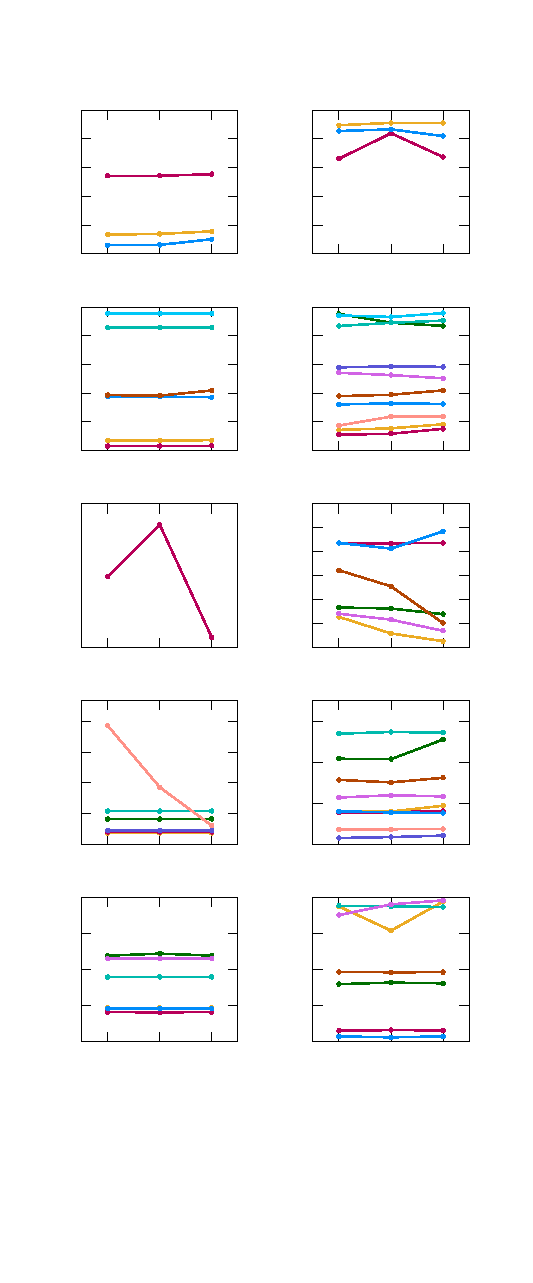
\includegraphics{./figures/parts/02/chapters/03/sections/04/simulations_pose_errors}}%
    \gplfronttext
  \end{picture}%
\endgroup

  \end{subfigure}\hspace{1.0cm}
  \begin{subfigure}{0.5\linewidth}
    % GNUPLOT: LaTeX picture with Postscript
\begingroup
  \makeatletter
  \providecommand\color[2][]{%
    \GenericError{(gnuplot) \space\space\space\@spaces}{%
      Package color not loaded in conjunction with
      terminal option `colourtext'%
    }{See the gnuplot documentation for explanation.%
    }{Either use 'blacktext' in gnuplot or load the package
      color.sty in LaTeX.}%
    \renewcommand\color[2][]{}%
  }%
  \providecommand\includegraphics[2][]{%
    \GenericError{(gnuplot) \space\space\space\@spaces}{%
      Package graphicx or graphics not loaded%
    }{See the gnuplot documentation for explanation.%
    }{The gnuplot epslatex terminal needs graphicx.sty or graphics.sty.}%
    \renewcommand\includegraphics[2][]{}%
  }%
  \providecommand\rotatebox[2]{#2}%
  \@ifundefined{ifGPcolor}{%
    \newif\ifGPcolor
    \GPcolorfalse
  }{}%
  \@ifundefined{ifGPblacktext}{%
    \newif\ifGPblacktext
    \GPblacktexttrue
  }{}%
  % define a \g@addto@macro without @ in the name:
  \let\gplgaddtomacro\g@addto@macro
  % define empty templates for all commands taking text:
  \gdef\gplfronttext{}%
  \gdef\gplfronttext{}%
  \makeatother
  \ifGPblacktext
    % no textcolor at all
    \def\colorrgb#1{}%
    \def\colorgray#1{}%
  \else
    % gray or color?
    \ifGPcolor
      \def\colorrgb#1{\color[rgb]{#1}}%
      \def\colorgray#1{\color[gray]{#1}}%
      \expandafter\def\csname LTw\endcsname{\color{white}}%
      \expandafter\def\csname LTb\endcsname{\color{black}}%
      \expandafter\def\csname LTa\endcsname{\color{black}}%
      \expandafter\def\csname LT0\endcsname{\color[rgb]{1,0,0}}%
      \expandafter\def\csname LT1\endcsname{\color[rgb]{0,1,0}}%
      \expandafter\def\csname LT2\endcsname{\color[rgb]{0,0,1}}%
      \expandafter\def\csname LT3\endcsname{\color[rgb]{1,0,1}}%
      \expandafter\def\csname LT4\endcsname{\color[rgb]{0,1,1}}%
      \expandafter\def\csname LT5\endcsname{\color[rgb]{1,1,0}}%
      \expandafter\def\csname LT6\endcsname{\color[rgb]{0,0,0}}%
      \expandafter\def\csname LT7\endcsname{\color[rgb]{1,0.3,0}}%
      \expandafter\def\csname LT8\endcsname{\color[rgb]{0.5,0.5,0.5}}%
    \else
      % gray
      \def\colorrgb#1{\color{black}}%
      \def\colorgray#1{\color[gray]{#1}}%
      \expandafter\def\csname LTw\endcsname{\color{white}}%
      \expandafter\def\csname LTb\endcsname{\color{black}}%
      \expandafter\def\csname LTa\endcsname{\color{black}}%
      \expandafter\def\csname LT0\endcsname{\color{black}}%
      \expandafter\def\csname LT1\endcsname{\color{black}}%
      \expandafter\def\csname LT2\endcsname{\color{black}}%
      \expandafter\def\csname LT3\endcsname{\color{black}}%
      \expandafter\def\csname LT4\endcsname{\color{black}}%
      \expandafter\def\csname LT5\endcsname{\color{black}}%
      \expandafter\def\csname LT6\endcsname{\color{black}}%
      \expandafter\def\csname LT7\endcsname{\color{black}}%
      \expandafter\def\csname LT8\endcsname{\color{black}}%
    \fi
  \fi
  \setlength{\unitlength}{0.0500bp}%
  \begin{picture}(4800.00,12000.00)%
    \gplgaddtomacro\gplfronttext{%
      \colorrgb{0.00,0.00,0.00}%
      \put(492,9720){\makebox(0,0)[r]{\strut{}\small $160$}}%
      \colorrgb{0.00,0.00,0.00}%
      \put(492,10065){\makebox(0,0)[r]{\strut{}\small $200$}}%
      \colorrgb{0.00,0.00,0.00}%
      \put(492,10410){\makebox(0,0)[r]{\strut{}\small $240$}}%
      \colorrgb{0.00,0.00,0.00}%
      \put(492,10754){\makebox(0,0)[r]{\strut{}\small $280$}}%
      \colorrgb{0.00,0.00,0.00}%
      \put(492,11099){\makebox(0,0)[r]{\strut{}\small $320$}}%
      \colorrgb{0.00,0.00,0.00}%
      \put(874,9500){\makebox(0,0){\strut{}}}%
      \colorrgb{0.00,0.00,0.00}%
      \put(1374,9500){\makebox(0,0){\strut{}}}%
      \colorrgb{0.00,0.00,0.00}%
      \put(1873,9500){\makebox(0,0){\strut{}}}%
      \colorrgb{0.00,0.00,0.00}%
      %\put(-410,10409){\rotatebox{90}{\makebox(0,0){\strut{}\small CORRIDOR}}}%
      \colorrgb{0.00,0.00,0.00}%
      \put(1373,11429){\makebox(0,0){\strut{}PLICP}}%
      \put(2500,11829){\makebox(0,0){\strut{}Χρόνος εκτέλεσης [ms]}}%
    }%
    \gplgaddtomacro\gplfronttext{%
    }%
    \gplgaddtomacro\gplfronttext{%
      \colorrgb{0.00,0.00,0.00}%
      \put(2712,9720){\makebox(0,0)[r]{\strut{}\small $160$}}%
      \colorrgb{0.00,0.00,0.00}%
      \put(2712,10065){\makebox(0,0)[r]{\strut{}\small $200$}}%
      \colorrgb{0.00,0.00,0.00}%
      \put(2712,10410){\makebox(0,0)[r]{\strut{}\small $240$}}%
      \colorrgb{0.00,0.00,0.00}%
      \put(2712,10754){\makebox(0,0)[r]{\strut{}\small $208$}}%
      \colorrgb{0.00,0.00,0.00}%
      \put(2712,11099){\makebox(0,0)[r]{\strut{}\small $320$}}%
      \colorrgb{0.00,0.00,0.00}%
      \put(3094,9500){\makebox(0,0){\strut{}}}%
      \colorrgb{0.00,0.00,0.00}%
      \put(3594,9500){\makebox(0,0){\strut{}}}%
      \colorrgb{0.00,0.00,0.00}%
      \put(4093,9500){\makebox(0,0){\strut{}}}%
      \colorrgb{0.00,0.00,0.00}%
      \put(3593,11429){\makebox(0,0){\strut{}PGL-FMIC}}%
    }%
    \gplgaddtomacro\gplfronttext{%
    }%
    \gplgaddtomacro\gplfronttext{%
      \colorrgb{0.00,0.00,0.00}%
      \put(492,7830){\makebox(0,0)[r]{\strut{}\small $160$}}%
      \colorrgb{0.00,0.00,0.00}%
      \put(492,8175){\makebox(0,0)[r]{\strut{}\small $240$}}%
      \colorrgb{0.00,0.00,0.00}%
      \put(492,8520){\makebox(0,0)[r]{\strut{}\small $320$}}%
      \colorrgb{0.00,0.00,0.00}%
      \put(492,8864){\makebox(0,0)[r]{\strut{}\small $400$}}%
      \colorrgb{0.00,0.00,0.00}%
      \put(492,9209){\makebox(0,0)[r]{\strut{}\small $480$}}%
      \colorrgb{0.00,0.00,0.00}%
      \put(874,7610){\makebox(0,0){\strut{}}}%
      \colorrgb{0.00,0.00,0.00}%
      \put(1374,7610){\makebox(0,0){\strut{}}}%
      \colorrgb{0.00,0.00,0.00}%
      \put(1873,7610){\makebox(0,0){\strut{}}}%
      \colorrgb{0.00,0.00,0.00}%
      %\put(-410,8519){\rotatebox{90}{\makebox(0,0){\strut{}\small HOME}}}%
    }%
    \gplgaddtomacro\gplfronttext{%
    }%
    \gplgaddtomacro\gplfronttext{%
      \colorrgb{0.00,0.00,0.00}%
      \put(2712,7830){\makebox(0,0)[r]{\strut{}\small $160$}}%
      \colorrgb{0.00,0.00,0.00}%
      \put(2712,8175){\makebox(0,0)[r]{\strut{}\small $240$}}%
      \colorrgb{0.00,0.00,0.00}%
      \put(2712,8520){\makebox(0,0)[r]{\strut{}\small $320$}}%
      \colorrgb{0.00,0.00,0.00}%
      \put(2712,8864){\makebox(0,0)[r]{\strut{}\small $400$}}%
      \colorrgb{0.00,0.00,0.00}%
      \put(2712,9209){\makebox(0,0)[r]{\strut{}\small $480$}}%
      \colorrgb{0.00,0.00,0.00}%
      \put(3094,7610){\makebox(0,0){\strut{}}}%
      \colorrgb{0.00,0.00,0.00}%
      \put(3594,7610){\makebox(0,0){\strut{}}}%
      \colorrgb{0.00,0.00,0.00}%
      \put(4093,7610){\makebox(0,0){\strut{}}}%
    }%
    \gplgaddtomacro\gplfronttext{%
    }%
    \gplgaddtomacro\gplfronttext{%
      \colorrgb{0.00,0.00,0.00}%
      \put(492,5940){\makebox(0,0)[r]{\strut{}\small $200$}}%
      \colorrgb{0.00,0.00,0.00}%
      \put(492,6400){\makebox(0,0)[r]{\strut{}\small $280$}}%
      \colorrgb{0.00,0.00,0.00}%
      \put(492,6859){\makebox(0,0)[r]{\strut{}\small $360$}}%
      \colorrgb{0.00,0.00,0.00}%
      \put(492,7319){\makebox(0,0)[r]{\strut{}\small $440$}}%
      \colorrgb{0.00,0.00,0.00}%
      \put(874,5720){\makebox(0,0){\strut{}}}%
      \colorrgb{0.00,0.00,0.00}%
      \put(1374,5720){\makebox(0,0){\strut{}}}%
      \colorrgb{0.00,0.00,0.00}%
      \put(1873,5720){\makebox(0,0){\strut{}}}%
      \colorrgb{0.00,0.00,0.00}%
      %\put(-410,6629){\rotatebox{90}{\makebox(0,0){\strut{}\small WAREHOUSE}}}%
    }%
    \gplgaddtomacro\gplfronttext{%
    }%
    \gplgaddtomacro\gplfronttext{%
      \colorrgb{0.00,0.00,0.00}%
      \put(2712,5940){\makebox(0,0)[r]{\strut{}\small $200$}}%
      \colorrgb{0.00,0.00,0.00}%
      \put(2712,6400){\makebox(0,0)[r]{\strut{}\small $280$}}%
      \colorrgb{0.00,0.00,0.00}%
      \put(2712,6859){\makebox(0,0)[r]{\strut{}\small $360$}}%
      \colorrgb{0.00,0.00,0.00}%
      \put(2712,7319){\makebox(0,0)[r]{\strut{}\small $440$}}%
      \colorrgb{0.00,0.00,0.00}%
      \put(3094,5720){\makebox(0,0){\strut{}}}%
      \colorrgb{0.00,0.00,0.00}%
      \put(3594,5720){\makebox(0,0){\strut{}}}%
      \colorrgb{0.00,0.00,0.00}%
      \put(4093,5720){\makebox(0,0){\strut{}}}%
    }%
    \gplgaddtomacro\gplfronttext{%
    }%
    \gplgaddtomacro\gplfronttext{%
      \colorrgb{0.00,0.00,0.00}%
      \put(492,4050){\makebox(0,0)[r]{\strut{}\small $50$}}%
      \colorrgb{0.00,0.00,0.00}%
      \put(492,4247){\makebox(0,0)[r]{\strut{}\small $100$}}%
      \colorrgb{0.00,0.00,0.00}%
      \put(492,4444){\makebox(0,0)[r]{\strut{}\small $150$}}%
      \colorrgb{0.00,0.00,0.00}%
      \put(492,4641){\makebox(0,0)[r]{\strut{}\small $200$}}%
      \colorrgb{0.00,0.00,0.00}%
      \put(492,4838){\makebox(0,0)[r]{\strut{}\small $250$}}%
      \colorrgb{0.00,0.00,0.00}%
      \put(492,5035){\makebox(0,0)[r]{\strut{}\small $300$}}%
      \colorrgb{0.00,0.00,0.00}%
      \put(492,5232){\makebox(0,0)[r]{\strut{}\small $350$}}%
      \colorrgb{0.00,0.00,0.00}%
      \put(492,5429){\makebox(0,0)[r]{\strut{}\small $400$}}%
      \colorrgb{0.00,0.00,0.00}%
      \put(874,3830){\makebox(0,0){\strut{}}}%
      \colorrgb{0.00,0.00,0.00}%
      \put(1374,3830){\makebox(0,0){\strut{}}}%
      \colorrgb{0.00,0.00,0.00}%
      \put(1873,3830){\makebox(0,0){\strut{}}}%
      \colorrgb{0.00,0.00,0.00}%
      %\put(-410,4739){\rotatebox{90}{\makebox(0,0){\strut{}\small WILLOWGARAGE}}}%
    }%
    \gplgaddtomacro\gplfronttext{%
    }%
    \gplgaddtomacro\gplfronttext{%
      \colorrgb{0.00,0.00,0.00}%
      \put(2712,4050){\makebox(0,0)[r]{\strut{}\small $50$}}%
      \colorrgb{0.00,0.00,0.00}%
      \put(2712,4247){\makebox(0,0)[r]{\strut{}\small $100$}}%
      \colorrgb{0.00,0.00,0.00}%
      \put(2712,4444){\makebox(0,0)[r]{\strut{}\small $150$}}%
      \colorrgb{0.00,0.00,0.00}%
      \put(2712,4641){\makebox(0,0)[r]{\strut{}\small $200$}}%
      \colorrgb{0.00,0.00,0.00}%
      \put(2712,4838){\makebox(0,0)[r]{\strut{}\small $250$}}%
      \colorrgb{0.00,0.00,0.00}%
      \put(2712,5035){\makebox(0,0)[r]{\strut{}\small $300$}}%
      \colorrgb{0.00,0.00,0.00}%
      \put(2712,5232){\makebox(0,0)[r]{\strut{}\small $350$}}%
      \colorrgb{0.00,0.00,0.00}%
      \put(2712,5429){\makebox(0,0)[r]{\strut{}\small $400$}}%
      \colorrgb{0.00,0.00,0.00}%
      \put(3094,3830){\makebox(0,0){\strut{}}}%
      \colorrgb{0.00,0.00,0.00}%
      \put(3594,3830){\makebox(0,0){\strut{}}}%
      \colorrgb{0.00,0.00,0.00}%
      \put(4093,3830){\makebox(0,0){\strut{}}}%
    }%
    \gplgaddtomacro\gplfronttext{%
    }%
    \gplgaddtomacro\gplfronttext{%
      \colorrgb{0.00,0.00,0.00}%
      \put(492,2160){\makebox(0,0)[r]{\strut{}\small $200$}}%
      \colorrgb{0.00,0.00,0.00}%
      \put(492,2620){\makebox(0,0)[r]{\strut{}\small $250$}}%
      \colorrgb{0.00,0.00,0.00}%
      \put(492,3079){\makebox(0,0)[r]{\strut{}\small $300$}}%
      \colorrgb{0.00,0.00,0.00}%
      \put(492,3539){\makebox(0,0)[r]{\strut{}\small $350$}}%
      \colorrgb{0.00,0.00,0.00}%
      \put(874,1940){\makebox(0,0){\strut{}\scriptsize  $0.01$}}%
      \colorrgb{0.00,0.00,0.00}%
      \put(1374,1940){\makebox(0,0){\strut{}\scriptsize  $0.02$}}%
      \colorrgb{0.00,0.00,0.00}%
      \put(1873,1940){\makebox(0,0){\strut{}\scriptsize  $0.05$}}%
      \colorrgb{0.00,0.00,0.00}%
      %\put(-410,2849){\rotatebox{90}{\makebox(0,0){\strut{}\small LANDFILL}}}%
      \colorrgb{0.00,0.00,0.00}%
      \put(2500,1610){\makebox(0,0){\strut{}\small $d$ [m]: Θόρυβος μέτρησης $\mathcal{N}(0.0,d)$}}%
    }%
    \gplgaddtomacro\gplfronttext{%
    }%
    \gplgaddtomacro\gplfronttext{%
      \colorrgb{0.00,0.00,0.00}%
      \put(2712,2160){\makebox(0,0)[r]{\strut{}\small $200$}}%
      \colorrgb{0.00,0.00,0.00}%
      \put(2712,2620){\makebox(0,0)[r]{\strut{}\small $250$}}%
      \colorrgb{0.00,0.00,0.00}%
      \put(2712,3079){\makebox(0,0)[r]{\strut{}\small $300$}}%
      \colorrgb{0.00,0.00,0.00}%
      \put(2712,3539){\makebox(0,0)[r]{\strut{}\small $350$}}%
      \colorrgb{0.00,0.00,0.00}%
      \put(3094,1940){\makebox(0,0){\strut{}\scriptsize $0.01$}}%
      \colorrgb{0.00,0.00,0.00}%
      \put(3594,1940){\makebox(0,0){\strut{}\scriptsize  $0.02$}}%
      \colorrgb{0.00,0.00,0.00}%
      \put(4093,1940){\makebox(0,0){\strut{}\scriptsize  $0.05$}}%
    }%
    \gplgaddtomacro\gplfronttext{%
    }%
    \put(0,0){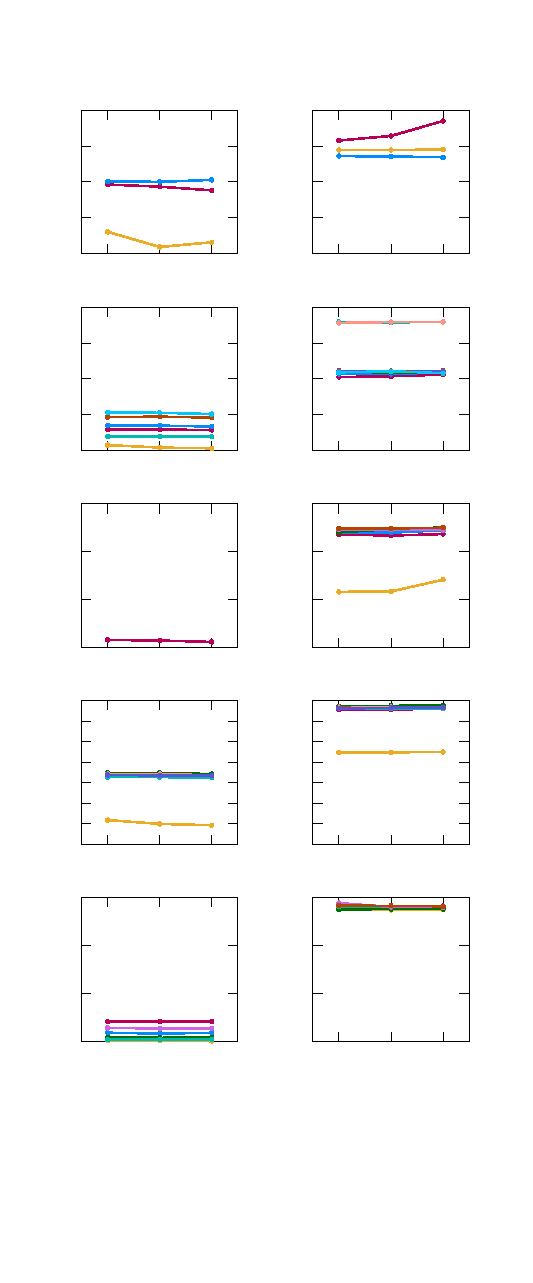
\includegraphics{./figures/parts/02/chapters/03/sections/04/simulations_execution_times}}%
    \gplfronttext
  \end{picture}%
\endgroup

  \end{subfigure}
  \vspace{-2.5cm}
  \caption{\small Μέση τιμή σφάλματος στάσης ορθών λύσεων (αριστερά) και μέση
           τιμή χρόνου εκτέλεσης ανά υπόθεση (δεξιά) ανά περιβάλλον
           προσομοίωσης, στάση, και τυπική απόκλιση θορύβου μέτρησης}
\label{fig:02_03_04:sim_pose_errors_and_exec_times}
\end{figure}

\begin{figure}[h]
  \hspace{1cm}
  \begin{subfigure}{0.5\linewidth}
    % GNUPLOT: LaTeX picture with Postscript
\begingroup
  \makeatletter
  \providecommand\color[2][]{%
    \GenericError{(gnuplot) \space\space\space\@spaces}{%
      Package color not loaded in conjunction with
      terminal option `colourtext'%
    }{See the gnuplot documentation for explanation.%
    }{Either use 'blacktext' in gnuplot or load the package
      color.sty in LaTeX.}%
    \renewcommand\color[2][]{}%
  }%
  \providecommand\includegraphics[2][]{%
    \GenericError{(gnuplot) \space\space\space\@spaces}{%
      Package graphicx or graphics not loaded%
    }{See the gnuplot documentation for explanation.%
    }{The gnuplot epslatex terminal needs graphicx.sty or graphics.sty.}%
    \renewcommand\includegraphics[2][]{}%
  }%
  \providecommand\rotatebox[2]{#2}%
  \@ifundefined{ifGPcolor}{%
    \newif\ifGPcolor
    \GPcolorfalse
  }{}%
  \@ifundefined{ifGPblacktext}{%
    \newif\ifGPblacktext
    \GPblacktexttrue
  }{}%
  % define a \g@addto@macro without @ in the name:
  \let\gplgaddtomacro\g@addto@macro
  % define empty templates for all commands taking text:
  \gdef\gplfronttext{}%
  \gdef\gplfronttext{}%
  \makeatother
  \ifGPblacktext
    % no textcolor at all
    \def\colorrgb#1{}%
    \def\colorgray#1{}%
  \else
    % gray or color?
    \ifGPcolor
      \def\colorrgb#1{\color[rgb]{#1}}%
      \def\colorgray#1{\color[gray]{#1}}%
      \expandafter\def\csname LTw\endcsname{\color{white}}%
      \expandafter\def\csname LTb\endcsname{\color{black}}%
      \expandafter\def\csname LTa\endcsname{\color{black}}%
      \expandafter\def\csname LT0\endcsname{\color[rgb]{1,0,0}}%
      \expandafter\def\csname LT1\endcsname{\color[rgb]{0,1,0}}%
      \expandafter\def\csname LT2\endcsname{\color[rgb]{0,0,1}}%
      \expandafter\def\csname LT3\endcsname{\color[rgb]{1,0,1}}%
      \expandafter\def\csname LT4\endcsname{\color[rgb]{0,1,1}}%
      \expandafter\def\csname LT5\endcsname{\color[rgb]{1,1,0}}%
      \expandafter\def\csname LT6\endcsname{\color[rgb]{0,0,0}}%
      \expandafter\def\csname LT7\endcsname{\color[rgb]{1,0.3,0}}%
      \expandafter\def\csname LT8\endcsname{\color[rgb]{0.5,0.5,0.5}}%
    \else
      % gray
      \def\colorrgb#1{\color{black}}%
      \def\colorgray#1{\color[gray]{#1}}%
      \expandafter\def\csname LTw\endcsname{\color{white}}%
      \expandafter\def\csname LTb\endcsname{\color{black}}%
      \expandafter\def\csname LTa\endcsname{\color{black}}%
      \expandafter\def\csname LT0\endcsname{\color{black}}%
      \expandafter\def\csname LT1\endcsname{\color{black}}%
      \expandafter\def\csname LT2\endcsname{\color{black}}%
      \expandafter\def\csname LT3\endcsname{\color{black}}%
      \expandafter\def\csname LT4\endcsname{\color{black}}%
      \expandafter\def\csname LT5\endcsname{\color{black}}%
      \expandafter\def\csname LT6\endcsname{\color{black}}%
      \expandafter\def\csname LT7\endcsname{\color{black}}%
      \expandafter\def\csname LT8\endcsname{\color{black}}%
    \fi
  \fi
  \setlength{\unitlength}{0.0500bp}%
  \begin{picture}(4000.00,3000.00)%
    \gplgaddtomacro\gplfronttext{%
      \colorrgb{0.00,0.00,0.00}%
      \put(388,1822){\makebox(0,0)[r]{\strut{}\small $0.0$}}%
      \colorrgb{0.00,0.00,0.00}%
      \put(388,2060){\makebox(0,0)[r]{\strut{}\small $0.10$}}%
      \colorrgb{0.00,0.00,0.00}%
      \put(388,2298){\makebox(0,0)[r]{\strut{}\small $0.20$}}%
      \colorrgb{0.00,0.00,0.00}%
      \put(388,2536){\makebox(0,0)[r]{\strut{}\small $0.30$}}%
      \colorrgb{0.00,0.00,0.00}%
      \put(388,2774){\makebox(0,0)[r]{\strut{}\small $0.40$}}%
      \colorrgb{0.00,0.00,0.00}%
      \put(778,1602){\makebox(0,0){\strut{}}}%
      \colorrgb{0.00,0.00,0.00}%
      \put(1037,1602){\makebox(0,0){\strut{}}}%
      \colorrgb{0.00,0.00,0.00}%
      \put(1295,1602){\makebox(0,0){\strut{}}}%
      \colorrgb{0.00,0.00,0.00}%
      \put(1553,1602){\makebox(0,0){\strut{}}}%
      \colorrgb{0.00,0.00,0.00}%
      \put(1811,1602){\makebox(0,0){\strut{}}}%
      \colorrgb{0.00,0.00,0.00}%
      \put(2070,1602){\makebox(0,0){\strut{}}}%
      \colorrgb{0.00,0.00,0.00}%
      \put(2328,1602){\makebox(0,0){\strut{}}}%
      \colorrgb{0.00,0.00,0.00}%
      \put(2586,1602){\makebox(0,0){\strut{}}}%
      \colorrgb{0.00,0.00,0.00}%
      \put(2844,1602){\makebox(0,0){\strut{}}}%
      \colorrgb{0.00,0.00,0.00}%
      \put(3103,1602){\makebox(0,0){\strut{}}}%
      \colorrgb{0.00,0.00,0.00}%
      \put(3361,1602){\makebox(0,0){\strut{}}}%
      \colorrgb{0.00,0.00,0.00}%
      \put(-646,2298){\rotatebox{90}{\makebox(0,0){\strut{}PLICP}}}%
      \colorrgb{0.00,0.00,0.00}%
      \put(2069,3104){\makebox(0,0){\strut{}Σφάλμα στάσης}}%
    }%
    \gplgaddtomacro\gplfronttext{%
    }%
    \gplgaddtomacro\gplfronttext{%
      \colorrgb{0.00,0.00,0.00}%
      \put(388,330){\makebox(0,0)[r]{\strut{}\small $0.0$}}%
      \colorrgb{0.00,0.00,0.00}%
      \put(388,568){\makebox(0,0)[r]{\strut{}\small $0.10$}}%
      \colorrgb{0.00,0.00,0.00}%
      \put(388,806){\makebox(0,0)[r]{\strut{}\small $0.20$}}%
      \colorrgb{0.00,0.00,0.00}%
      \put(388,1044){\makebox(0,0)[r]{\strut{}\small $0.30$}}%
      \colorrgb{0.00,0.00,0.00}%
      \put(388,1282){\makebox(0,0)[r]{\strut{}\small $0.40$}}%
      \colorrgb{0.00,0.00,0.00}%
      \put(778,110){\makebox(0,0){\strut{}\small $\bm{p}_a^A$}}%
      \colorrgb{0.00,0.00,0.00}%
      \put(1037,110){\makebox(0,0){\strut{}\small $\bm{p}_b^A$}}%
      \colorrgb{0.00,0.00,0.00}%
      \put(1295,110){\makebox(0,0){\strut{}\small $\bm{p}_c^A$}}%
      \colorrgb{0.00,0.00,0.00}%
      \put(1553,110){\makebox(0,0){\strut{}\small $\bm{p}_d^A$}}%
      \colorrgb{0.00,0.00,0.00}%
      \put(1811,110){\makebox(0,0){\strut{}\small $\bm{p}_e^A$}}%
      \colorrgb{0.00,0.00,0.00}%
      \put(2070,110){\makebox(0,0){\strut{}\small $\bm{p}_f^A$}}%
      \colorrgb{0.00,0.00,0.00}%
      \put(2328,110){\makebox(0,0){\strut{}\small $\bm{p}_g^A$}}%
      \colorrgb{0.00,0.00,0.00}%
      \put(2586,110){\makebox(0,0){\strut{}\small $\bm{p}_h^A$}}%
      \colorrgb{0.00,0.00,0.00}%
      \put(2844,110){\makebox(0,0){\strut{}\small $\bm{p}_i^A$}}%
      \colorrgb{0.00,0.00,0.00}%
      \put(3103,110){\makebox(0,0){\strut{}\small $\bm{p}_j^A$}}%
      \colorrgb{0.00,0.00,0.00}%
      \put(3361,110){\makebox(0,0){\strut{}\small $\bm{p}_k^A$}}%
      \colorrgb{0.00,0.00,0.00}%
      \put(-646,806){\rotatebox{90}{\makebox(0,0){\strut{}PGL-FMIC}}}%
      \colorrgb{0.00,0.00,0.00}%
      \put(2069,-220){\makebox(0,0){\strut{}Σημαίνον στάσης}}%
    }%
    \gplgaddtomacro\gplfronttext{%
    }%
    \put(0,0){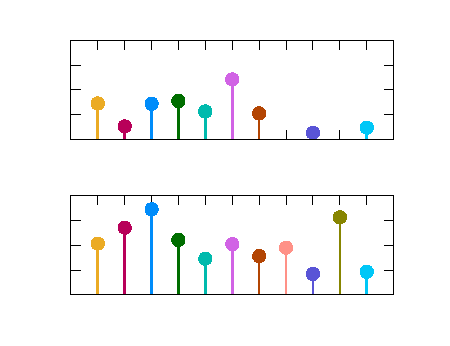
\includegraphics{./figures/parts/02/chapters/03/sections/04/csal_pose_errors}}%
    \gplfronttext
  \end{picture}%
\endgroup

  \end{subfigure}%
  \begin{subfigure}{0.5\linewidth}
    % GNUPLOT: LaTeX picture with Postscript
\begingroup
  \makeatletter
  \providecommand\color[2][]{%
    \GenericError{(gnuplot) \space\space\space\@spaces}{%
      Package color not loaded in conjunction with
      terminal option `colourtext'%
    }{See the gnuplot documentation for explanation.%
    }{Either use 'blacktext' in gnuplot or load the package
      color.sty in LaTeX.}%
    \renewcommand\color[2][]{}%
  }%
  \providecommand\includegraphics[2][]{%
    \GenericError{(gnuplot) \space\space\space\@spaces}{%
      Package graphicx or graphics not loaded%
    }{See the gnuplot documentation for explanation.%
    }{The gnuplot epslatex terminal needs graphicx.sty or graphics.sty.}%
    \renewcommand\includegraphics[2][]{}%
  }%
  \providecommand\rotatebox[2]{#2}%
  \@ifundefined{ifGPcolor}{%
    \newif\ifGPcolor
    \GPcolorfalse
  }{}%
  \@ifundefined{ifGPblacktext}{%
    \newif\ifGPblacktext
    \GPblacktexttrue
  }{}%
  % define a \g@addto@macro without @ in the name:
  \let\gplgaddtomacro\g@addto@macro
  % define empty templates for all commands taking text:
  \gdef\gplfronttext{}%
  \gdef\gplfronttext{}%
  \makeatother
  \ifGPblacktext
    % no textcolor at all
    \def\colorrgb#1{}%
    \def\colorgray#1{}%
  \else
    % gray or color?
    \ifGPcolor
      \def\colorrgb#1{\color[rgb]{#1}}%
      \def\colorgray#1{\color[gray]{#1}}%
      \expandafter\def\csname LTw\endcsname{\color{white}}%
      \expandafter\def\csname LTb\endcsname{\color{black}}%
      \expandafter\def\csname LTa\endcsname{\color{black}}%
      \expandafter\def\csname LT0\endcsname{\color[rgb]{1,0,0}}%
      \expandafter\def\csname LT1\endcsname{\color[rgb]{0,1,0}}%
      \expandafter\def\csname LT2\endcsname{\color[rgb]{0,0,1}}%
      \expandafter\def\csname LT3\endcsname{\color[rgb]{1,0,1}}%
      \expandafter\def\csname LT4\endcsname{\color[rgb]{0,1,1}}%
      \expandafter\def\csname LT5\endcsname{\color[rgb]{1,1,0}}%
      \expandafter\def\csname LT6\endcsname{\color[rgb]{0,0,0}}%
      \expandafter\def\csname LT7\endcsname{\color[rgb]{1,0.3,0}}%
      \expandafter\def\csname LT8\endcsname{\color[rgb]{0.5,0.5,0.5}}%
    \else
      % gray
      \def\colorrgb#1{\color{black}}%
      \def\colorgray#1{\color[gray]{#1}}%
      \expandafter\def\csname LTw\endcsname{\color{white}}%
      \expandafter\def\csname LTb\endcsname{\color{black}}%
      \expandafter\def\csname LTa\endcsname{\color{black}}%
      \expandafter\def\csname LT0\endcsname{\color{black}}%
      \expandafter\def\csname LT1\endcsname{\color{black}}%
      \expandafter\def\csname LT2\endcsname{\color{black}}%
      \expandafter\def\csname LT3\endcsname{\color{black}}%
      \expandafter\def\csname LT4\endcsname{\color{black}}%
      \expandafter\def\csname LT5\endcsname{\color{black}}%
      \expandafter\def\csname LT6\endcsname{\color{black}}%
      \expandafter\def\csname LT7\endcsname{\color{black}}%
      \expandafter\def\csname LT8\endcsname{\color{black}}%
    \fi
  \fi
  \setlength{\unitlength}{0.0500bp}%
  \begin{picture}(4000.00,3000.00)%
    \gplgaddtomacro\gplfronttext{%
      \colorrgb{0.00,0.00,0.00}%
      \put(388,1822){\makebox(0,0)[r]{\strut{}\small $0$}}%
      \colorrgb{0.00,0.00,0.00}%
      \put(388,1981){\makebox(0,0)[r]{\strut{}\small $200$}}%
      \colorrgb{0.00,0.00,0.00}%
      \put(388,2139){\makebox(0,0)[r]{\strut{}\small $400$}}%
      \colorrgb{0.00,0.00,0.00}%
      \put(388,2298){\makebox(0,0)[r]{\strut{}\small $600$}}%
      \colorrgb{0.00,0.00,0.00}%
      \put(388,2457){\makebox(0,0)[r]{\strut{}\small $800$}}%
      \colorrgb{0.00,0.00,0.00}%
      \put(388,2615){\makebox(0,0)[r]{\strut{}\small $1000$}}%
      \colorrgb{0.00,0.00,0.00}%
      \put(388,2774){\makebox(0,0)[r]{\strut{}\small $1200$}}%
      \colorrgb{0.00,0.00,0.00}%
      \put(778,1602){\makebox(0,0){\strut{}}}%
      \colorrgb{0.00,0.00,0.00}%
      \put(1037,1602){\makebox(0,0){\strut{}}}%
      \colorrgb{0.00,0.00,0.00}%
      \put(1295,1602){\makebox(0,0){\strut{}}}%
      \colorrgb{0.00,0.00,0.00}%
      \put(1553,1602){\makebox(0,0){\strut{}}}%
      \colorrgb{0.00,0.00,0.00}%
      \put(1811,1602){\makebox(0,0){\strut{}}}%
      \colorrgb{0.00,0.00,0.00}%
      \put(2070,1602){\makebox(0,0){\strut{}}}%
      \colorrgb{0.00,0.00,0.00}%
      \put(2328,1602){\makebox(0,0){\strut{}}}%
      \colorrgb{0.00,0.00,0.00}%
      \put(2586,1602){\makebox(0,0){\strut{}}}%
      \colorrgb{0.00,0.00,0.00}%
      \put(2844,1602){\makebox(0,0){\strut{}}}%
      \colorrgb{0.00,0.00,0.00}%
      \put(3103,1602){\makebox(0,0){\strut{}}}%
      \colorrgb{0.00,0.00,0.00}%
      \put(3361,1602){\makebox(0,0){\strut{}}}%
      \colorrgb{0.00,0.00,0.00}%
      %\put(-646,2298){\rotatebox{90}{\makebox(0,0){\strut{}PLICP}}}%
      \colorrgb{0.00,0.00,0.00}%
      \put(2069,3104){\makebox(0,0){\strut{}Χρόνος εκτέλεσης [ms]}}%
    }%
    \gplgaddtomacro\gplfronttext{%
    }%
    \gplgaddtomacro\gplfronttext{%
      \colorrgb{0.00,0.00,0.00}%
      \put(388,330){\makebox(0,0)[r]{\strut{}\small $0$}}%
      \colorrgb{0.00,0.00,0.00}%
      \put(388,489){\makebox(0,0)[r]{\strut{}\small $200$}}%
      \colorrgb{0.00,0.00,0.00}%
      \put(388,647){\makebox(0,0)[r]{\strut{}\small $400$}}%
      \colorrgb{0.00,0.00,0.00}%
      \put(388,806){\makebox(0,0)[r]{\strut{}\small $600$}}%
      \colorrgb{0.00,0.00,0.00}%
      \put(388,965){\makebox(0,0)[r]{\strut{}\small $800$}}%
      \colorrgb{0.00,0.00,0.00}%
      \put(388,1123){\makebox(0,0)[r]{\strut{}\small $1000$}}%
      \colorrgb{0.00,0.00,0.00}%
      \put(388,1282){\makebox(0,0)[r]{\strut{}\small $1200$}}%
      \colorrgb{0.00,0.00,0.00}%
      \put(778,110){\makebox(0,0){\strut{}\small $\bm{p}_a^A$}}%
      \colorrgb{0.00,0.00,0.00}%
      \put(1037,110){\makebox(0,0){\strut{}\small $\bm{p}_b^A$}}%
      \colorrgb{0.00,0.00,0.00}%
      \put(1295,110){\makebox(0,0){\strut{}\small $\bm{p}_c^A$}}%
      \colorrgb{0.00,0.00,0.00}%
      \put(1553,110){\makebox(0,0){\strut{}\small $\bm{p}_d^A$}}%
      \colorrgb{0.00,0.00,0.00}%
      \put(1811,110){\makebox(0,0){\strut{}\small $\bm{p}_e^A$}}%
      \colorrgb{0.00,0.00,0.00}%
      \put(2070,110){\makebox(0,0){\strut{}\small $\bm{p}_f^A$}}%
      \colorrgb{0.00,0.00,0.00}%
      \put(2328,110){\makebox(0,0){\strut{}\small $\bm{p}_g^A$}}%
      \colorrgb{0.00,0.00,0.00}%
      \put(2586,110){\makebox(0,0){\strut{}\small $\bm{p}_h^A$}}%
      \colorrgb{0.00,0.00,0.00}%
      \put(2844,110){\makebox(0,0){\strut{}\small $\bm{p}_i^A$}}%
      \colorrgb{0.00,0.00,0.00}%
      \put(3103,110){\makebox(0,0){\strut{}\small $\bm{p}_j^A$}}%
      \colorrgb{0.00,0.00,0.00}%
      \put(3361,110){\makebox(0,0){\strut{}\small $\bm{p}_k^A$}}%
      \colorrgb{0.00,0.00,0.00}%
      %\put(-646,806){\rotatebox{90}{\makebox(0,0){\strut{}PGL-FMIC}}}%
      \colorrgb{0.00,0.00,0.00}%
      \put(2069,-220){\makebox(0,0){\strut{}Σημαίνον στάσης}}%
    }%
    \gplgaddtomacro\gplfronttext{%
    }%
    \put(0,0){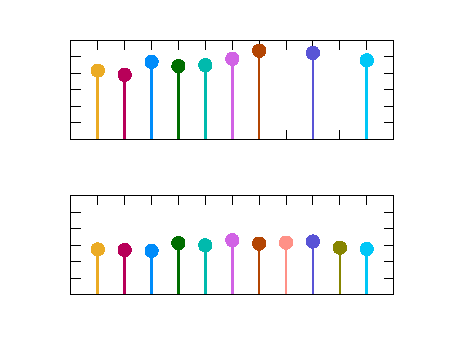
\includegraphics{./figures/parts/02/chapters/03/sections/04/csal_execution_times}}%
    \gplfronttext
  \end{picture}%
\endgroup

  \end{subfigure}
  \vspace{1cm}
\caption{\small Μέση τιμή σφάλματος στάσης ορθών λύσεων (αριστερά) και μέση
         τιμή χρόνου εκτέλεσης ανά υπόθεση (δεξιά) ανά στάση στο περιβάλλον
         CSAL}
\label{fig:02_03_04:csal_pose_errors_and_exec_times}
\end{figure}

%%%%%%%%%%%%%%%%%%%%%%%%%%%%%%%%%%%%%%%%%%%%%%%%%%%%%%%%%%%%%%%%%%%%%%%%%%%%%%%%
\subsection{Αξιολόγηση}
\label{subsection:02_03_04:03}

Όσον αφορά τα μεγέθη των σφαλμάτων εκτίμησης των δύο μεθόδων, δεν υπάρχει σαφής
μοτίβο κυριαρχίας του ενός αλγορίθμου έναντι του άλλου, και, δεδομένου του
μικρότερου μεγέθους μεταβλητών των οποίων η τιμή πρέπει να καθοριστεί, η
υπόθεση \ref{hypothesis:02_03:01} ευσταθεί: η μέθοδος FMIC δεν χρησιμοποιεί
τον υπολογισμό αντιστοιχίσεων για την ευθυγράμμιση πραγματικών και εικονικών
δισδιάστατων σαρώσεων, και εμφανίζει παρόμοια σφάλματα στάσης με την καλύτερη
μέθοδο ευθυγράμμισης πραγματικών με εικονικές σαρώσεις, PLICP.

Για τον PGL-FMIC το μέγιστο σφάλμα θέσης ήταν $0.45$ m, και εξαρτάται, όπως και
για τον PLICP, από τη γεωμετρία του περιβάλλοντος γύρω από την πραγματική στάση
του ρομπότ.  Ο καθαρός χρόνος εκτέλεσής του προτεινόμενου συστήματος ήταν
περίπου $50\%$ μεγαλύτερος από τον ολικό χρόνο εκτέλεσης του PLICP για χαμηλό
αριθμό ακτίνων αισθητήρων ($720$). H σχέση αυτή αντιστρέφεται όταν ο αριθμός
των ακτίνων τριπλασιάζεται σε μέγεθος (περιβάλλον CSAL).

Η μεγάλη διαφορά μεταξύ των επιδόσεων των δύο μεθόδων αποκαλύπτεται στο επίπεδο
των ορθών λύσεων (σχήμα \ref{fig:02_03_04:outliers}). Οι εκτιμήσεις του
PGL-FMIC περιλαμβάνουν μικρότερο αριθμό άκυρων λύσεων από εκείνες του PLICP.
Στο περιβάλλον CORRIDOR ο πρώτος παρήγαγε μία μη έγκυρη λύση σε
$3\times4\times100 = 1200$  προσομοιώσεις, ενώ ο PLICP απέτυχε περίπου σε μία
στις τέσσερις προσπάθειες επίλυσης του προβλήματος όταν το ρομπότ ήταν
τοποθετημένο στο σημείο $\bm{p}_b^C$, μη μπορώντας να διακρίνει μεταξύ του δύο
σχεδόν πανομοιότυπων διακλαδώσεων του περιβάλλοντος. Η επανάληψη της γεωμετρίας
του περιβάλλοντος γύρω από τη στάση $\bm{p}_j^H$ στο περιβάλλον HOME προκάλεσε
την αποτυχία και των δύο αλγορίθμων να εντοπίσουν το ρομπότ.

Στο περιβάλλον WAREHOUSE η ανεπάρκεια της μέγιστης εμβέλειας του αισθητήρα
αποστάσεων σε σχέση με τις αποστάσεις μεταξύ των αντικειμένων του περιβάλλοντος
είχε ως αποτέλεσμα ο PLICP να μην είναι σε θέση να εντοπίσει το ρομπότ για όλες
τις στάσεις εκτός από μία. Συγκριτικά, ο PGL-FMIC επηρεάστηκε λιγότερο από την
επίδραση των ελλιπών πληροφοριών, αδυνατώντας να εντοπίσει το ρομπότ μόνο όταν
η στάση του ήταν η $\bm{p}_e^W$.  Στο περιβάλλον WILLOWGARAGE ο PLICP δεν
μπόρεσε να εντοπίσει το ρομπότ για τέσσερις από τις δέκα στάσεις που
δοκιμάστηκαν. Για αυτές τις τέσσερις στάσεις μόνο ένας περιορισμένος αριθμός
ακτίνων έφερε ελλιπείς πληροφορίες.  Ίσως αυτό το αποτέλεσμα, σε συνδυασμό με
την εικασία ότι οι ακτίνες που φέρουν ελλιπείς πληροφορίες πρέπει να
αποκλειστούν από τον υπολογισμό αντιστοιχίσεων---και επομένως ότι οι παράμετροι
που σχετίζονται με την απόρριψη ακραίων τιμών πρέπει να ρυθμιστούν
αναλόγως---οδήγησε στην ανεπάρκεια του PLICP σε αυτό το περιβάλλον. Κατά
συνέπεια, εάν εφαρμοστεί η ίδια λογική, το ίδιο θα μπορούσε να ειπωθεί και για
τις προσομοιώσεις στο περιβάλλον WAREHOUSE, ωστόσο, ο στόχος μας εδώ είναι να
αποφύγουμε τον καθορισμό παραμέτρων με ad hoc τρόπο ή σε βάση ανά-τοποθεσία ή
περιβάλλον, όπως εξηγείται στην ενότητα \ref{subsection:02_02_05:02}.
Αντιθέτως, ο PGL-FMIC δεν μπόρεσε να εντοπίσει το ρομπότ μόνο σε μία περίπτωση
($\bm{p}_j^G$), για την οποία και οι δύο αλγόριθμοι δεν μπόρεσαν να επιλύσουν
την οκταπλή ασάφεια του περιβάλλοντος χώρου της πραγματικής στάσης. Δεδομένου
ότι τα αποτελέσματα για αυτό το περιβάλλον, όπου η ανάλυση του χάρτη είναι πιο
χονδροειδής από ό,τι στις τρεις περιπτώσεις που προηγήθηκαν, δεν υπάρχουν
στοιχεία που να υποστηρίζουν ότι η μεταβολή της ανάλυσης επιδεινώνει (ή
βελτιώνει) τις εκτιμήσεις των δύο μεθόδων.  Στο περιβάλλον LANDFILL ο PGL-FMIC
παρουσίασε ξανά λιγότερες άκυρες λύσεις από τον PLICP.  Η μη δομημένη φύση του
περιβάλλοντος επηρέασε την απόδοση της PGL-FMIC περισσότερο από τα άλλα
(δομημένα) περιβάλλοντα---περισσότερο όσον αφορά στα σφάλματα θέσης και
λιγότερο στα σφάλματα προσανατολισμού του.

Στο πραγματικό περιβάλλον του CSAL τα μέσα σφάλματα θέσης και προσανατολισμού
του PGL-FMIC δεν ξεπέρασαν τα $0.35$ m και $0.11$ rad αντίστοιχα. Όσον
αφορά στους χρόνους εκτέλεσης, αυτοί ήταν αυξημένοι και για τις δύο
μεθόδους λόγω του αυξημένου αριθμού ακτίνων του αισθητήρα YDLIDAR
σε σύγκριση με αυτόν του αισθητήρα που χρησιμοποιήθηκε στις προσομοιώσεις
($2019$ έναντι $720$). Οι χρόνοι της προτεινόμενης μεθόδου ήταν αυξημένοι
κατά περίπου δύο φορές, ενώ οι χρόνοι της PLICP αυξήθηκαν κατά τέσσερις φορές.
Κατά συνέπεια, συμπεραίνουμε ότι ο χρόνος εκτέλεσης του PGL-FMIC είναι ανάλογος
του αριθμού των ακτίνων του αισθητήρα απόστασης, ενώ παρουσιάζει ασθενέστερη
εξάρτηση από αυτόν σε σύγκριση με τον PLICP.

Συνολικά, όσον αφορά στα κριτήρια διάκρισης λύσεων---ο συντελεστής κλίμακας
$\sigma$ και ο βαθμός ομοιότητας $w$---, αυτά επέδειξαν, εντός λογικών ορίων,
συνεπή και ορθή συμπεριφορά διαχωρισμού μεταξύ της ορθότητας εκτίμησης
υποθέσεων στάσης. Η αποτυχία του PGL-FMIC όσον αφορά στις ορθές λύσεις
οφείλεται α) στην αποτυχία επίλυσης της ασάφειας σε ό,τι αφορά πανομοιότυπα ή
παρόμοια περιβάλλοντα, β) στην μεγάλη έλλειψη πληροφοριών απόστασης και γ) στον
υπερβολικό θόρυβο μετρήσεων.
